\documentclass[]{article}
\usepackage{lmodern}
\usepackage{amssymb,amsmath}
\usepackage{ifxetex,ifluatex}
\usepackage{fixltx2e} % provides \textsubscript
\ifnum 0\ifxetex 1\fi\ifluatex 1\fi=0 % if pdftex
  \usepackage[T1]{fontenc}
  \usepackage[utf8]{inputenc}
\else % if luatex or xelatex
  \ifxetex
    \usepackage{mathspec}
  \else
    \usepackage{fontspec}
  \fi
  \defaultfontfeatures{Ligatures=TeX,Scale=MatchLowercase}
\fi
% use upquote if available, for straight quotes in verbatim environments
\IfFileExists{upquote.sty}{\usepackage{upquote}}{}
% use microtype if available
\IfFileExists{microtype.sty}{%
\usepackage{microtype}
\UseMicrotypeSet[protrusion]{basicmath} % disable protrusion for tt fonts
}{}
\usepackage[margin=1in]{geometry}
\usepackage{hyperref}
\hypersetup{unicode=true,
            pdftitle={Submarine Cable Analysis for US Marine Renewable Energy Development},
            pdfauthor={Benjamin D. Best 1; Levi F. Kilcher 2},
            pdfborder={0 0 0},
            breaklinks=true}
\urlstyle{same}  % don't use monospace font for urls
\usepackage{longtable,booktabs}
\usepackage{graphicx,grffile}
\makeatletter
\def\maxwidth{\ifdim\Gin@nat@width>\linewidth\linewidth\else\Gin@nat@width\fi}
\def\maxheight{\ifdim\Gin@nat@height>\textheight\textheight\else\Gin@nat@height\fi}
\makeatother
% Scale images if necessary, so that they will not overflow the page
% margins by default, and it is still possible to overwrite the defaults
% using explicit options in \includegraphics[width, height, ...]{}
\setkeys{Gin}{width=\maxwidth,height=\maxheight,keepaspectratio}
\IfFileExists{parskip.sty}{%
\usepackage{parskip}
}{% else
\setlength{\parindent}{0pt}
\setlength{\parskip}{6pt plus 2pt minus 1pt}
}
\setlength{\emergencystretch}{3em}  % prevent overfull lines
\providecommand{\tightlist}{%
  \setlength{\itemsep}{0pt}\setlength{\parskip}{0pt}}
\setcounter{secnumdepth}{5}
% Redefines (sub)paragraphs to behave more like sections
\ifx\paragraph\undefined\else
\let\oldparagraph\paragraph
\renewcommand{\paragraph}[1]{\oldparagraph{#1}\mbox{}}
\fi
\ifx\subparagraph\undefined\else
\let\oldsubparagraph\subparagraph
\renewcommand{\subparagraph}[1]{\oldsubparagraph{#1}\mbox{}}
\fi

%%% Use protect on footnotes to avoid problems with footnotes in titles
\let\rmarkdownfootnote\footnote%
\def\footnote{\protect\rmarkdownfootnote}

%%% Change title format to be more compact
\usepackage{titling}

% Create subtitle command for use in maketitle
\newcommand{\subtitle}[1]{
  \posttitle{
    \begin{center}\large#1\end{center}
    }
}

\setlength{\droptitle}{-2em}
  \title{Submarine Cable Analysis for US Marine Renewable Energy Development}
  \pretitle{\vspace{\droptitle}\centering\huge}
  \posttitle{\par}
  \author{Benjamin D. Best \textsuperscript{1} \\ Levi F. Kilcher \textsuperscript{2}}
  \preauthor{\centering\large\emph}
  \postauthor{\par}
  \predate{\centering\large\emph}
  \postdate{\par}
  \date{2018-01-31\\
\textsuperscript{1}: EcoQuants, Santa Barbara, CA\\
\textsuperscript{2}: National Renewable Energy Lab, Golden, CO \newline}


\begin{document}
\maketitle

{
\setcounter{tocdepth}{4}
\tableofcontents
}
\listoffigures
\hypertarget{executive-summary}{%
\section*{Executive Summary}\label{executive-summary}}
\addcontentsline{toc}{section}{Executive Summary}

Marine energy (offshore wind, tidal, wave) have the potential to help
diversify the U.S. renewable energy portfolio, which is important to
reducing reliance on foreign non-renewable energy sources, powering the
U.S. economy in the 21st century, creating jobs, and to reducing
greenhouse gas emissions that contribute to climate change. The first
U.S. commercial marine energy facility went into production in December
of 2016: the Block Island (Rhode Island) offshore wind farm. As
implementation costs for these technologies continue to drop and
increasingly ambitious targets for renewable energy are set, marine
renewable energy planning and development will need to effectively
evaluate competing ocean uses. Marine renewable energy may be
complementary to other large scale renewables by offering consistent
energy in high demand times during morning and evening hours when solar
is less available and in proximity to coastal areas where populations
tend to concentrate (Gilman et al. 2016; Lehmann et al. 2017).

Operation and maintenance of submarine cables may conflict with marine
renewable energy development. The submarine cable industry handles 95\%
of inter-continental internet, data and voice traffic (Communications
Security, Reliability and Interoperability Council IV 2014), and is thus
vital to the US and global economy. Repair and maintenance of cables
traditionally involves grappling the cable and floating it to the
surface, so allowance for drift of the repairing vessel and laying down
of the additional splice of cable is dependent on bottom depth. Although
submarine cable locations are publicly accessible through electronic
navigation charts, a clear understanding of the areas where cable paths
compete with promising marine energy sites does not yet exist.

We applied industry-advised safety buffers (`setback' distances) to map
the areas where the cable industry is a stakeholder. This was done using
two setback widths: a twice-depth (`2z') buffer for new ``facilities'',
and a three-times depth (`3z') for new ``cables'' to prevent overlap of
bights for newly spliced cable material. Both of these buffers have a
minimum 500 m buffer on either side. Of the original 230,835 km of cable
in the ``NOAA Charted Submarine cables in the United States as of
December 2012'' dataset (Figure \ref{fig:mapCableTerritories}), 97,321
km fell within the 200 nm of the US exclusive economic zone (EEZ), which
was analyzed across 12 territories that overlapped with the cables
(Figure \ref{fig:mapCableTerritories}). The cable buffer area ranged
from 29.35\% (242,031 km\textsuperscript{2} {[}3z{]} of 824,679
km\textsuperscript{2} total) along the West owing to many cables present
and the steep continental shelf, to virtually nill 0.39\% (6,133
km\textsuperscript{2} {[}2z{]} of 1,553,288 km\textsuperscript{2} total)
in the Gulf of Mexico (Table 2).

Overlap of cable buffers with marine renewable energy was assessed for
tidal (Haas et al. 2011), wave (Jacobson et al. 2011) and wind (Schwartz
et al. 2010) energy based on energy resource characterizations available
through the National Renewable Energy Lab (NREL) Wind
Prospector\footnote{NREL Wind Prospector:
  \url{https://maps.nrel.gov/wind-prospector/}} or MHK Atlas\footnote{NREL
  MHK Atlas: \url{https://maps.nrel.gov/mhk-atlas}}. Assessment of
overlap with the advised separation schemes and energy resource was
limited to maximum depths based on current assessment of technology
limitations : \textless{} 100 m for tidal (Haas et al. 2011),
\textless{} 200 m for wave (Jacobson et al. 2011), \textless{} 1,000 m
for wind (Musial et al. 2016). The lowest energy classes were also
dropped from the assessment (tidal: \textgreater{} 500 \(W/m^2\), wave:
\textgreater{} 10 \(kW/m\), wind: \textgreater{} 7 \(m/s\)) viable for
energy development.

Total area of viable tidal resource (1,671 \(km^2\)) is orders of
magnitude less than wave (378,908 \(km^2\)) or wind (462,613 \(km^2\))
owing to requirements for channelized bathymetry (Table 2). Nationally,
tidal energy has up to 3.8\% overlap, wave 0.9\% and wind 4\% (Table 2),
so conflict between viable marine renewable energy resource and existing
submarine cables is generally minimal. However a small fraction of
viable resource areas in high energy areas is notable. For instance, for
the small area (207 \(km^2\)) of highest wind speeds (11-12 m/s)
occurring only in Hawaii overlap is up to 37.9\% (Table 6). The lowest
tidal energy class (500 - 1,000 \(W/m^2\)) in the West region (11
\(km^2\)), largely around Puget Sound, has 31.5\% overlap (Table 4). The
report provides a detailed breakdown of overlap with energy resource by
depth, energy class and territory.

Energy resources are unevenly distributed across territories. Tidal
power (Table 4) is most abundant in Alaska (691 \(km^2\) at 500 - 1,000
\(W/m^2\)), the East (390 \(km^2\) at 500 - 1,000 \(W/m^2\)) and the
West (46 \(km^2\) at 500 - 1,000 \(W/m^2\)), which is where overlap with
cable buffers is most significant (23.4 - 31.5\%) such as around Port
Townsend, WA (Figure \ref{fig:mapTideWest}). Wave energy (Table 5) is
most abundant in the Pacific territories having the most exposure to
storm activity across the largest ocean. Alaska has the most abundant
energy across all viable energy classes. Wind speeds (Table 6) in excess
of 9 \(m/s\) are not found in the Gulf of Mexico and limited to the
offshore New England area of the East (Figure \ref{fig:mapWindEast}),
offshore areas of California and Oregon in the West (Figure
\ref{fig:mapWindEast}) and dispersed locations in Hawaii (Figure
\ref{fig:mapWindEast}).

The proposed avoidance areas for submarine cables should be deemed
advisory. Overlap with the new facility (3z) or cable (2z) buffers
around existing submarine cables does not nullify the possibility of
renewable energy development there. Rather, it should alert the
developer to negotiate reasonable terms with the cable operator via
contacting the cable industry, such as the North American Submarine
Cable Association\footnote{North American Submarine Cable Association
  (NASCA): \url{https://www.n-a-s-c-a.org}} or the International Cable
Protection Committee\footnote{International Cable Protection Committee
  (ICPC): \url{https://www.iscpc.org}}. These avoidance zones are
advised according to traditional methods of submarine cable repair
involving grappling of the submarine cable and buoying to the surface
for repair, hence allowance for sway of boat as a function of depth. In
future, use of more sophisticated remotely operated vehicles may narrow
safe operating distances. These avoidance areas are limited to the most
recent submarine cable data. Any planning for marine renewable energy
should consult the latest electronic navigation charts and contact the
cable industry for confirmation.

\hypertarget{background}{%
\section{Background}\label{background}}

Demand for abundant and diverse resources in the oceans is growing,
necessitating marine spatial planning. To inform development of Marine
Hydrokinetic (MHK) and Offshore Wind (OSW) resources, the Department of
Energy (DOE) has asked NREL to identify the competing uses areas between
promising MHK/OSW sites and submarine power and telecommunications
cables. The first step in this work is to identify and quantify the
overlap between the MHK/OSW resource availability and existing cable
routes.

The analysis is done in terms of resource area because the task of
quantifying actual impacts on available resource is a non-trivial
undertaking that involves subjective decisions of identifying resource
opportunities. Quantifying overlap in-terms of resource area---on the
other hand---is significantly more straight forward, and useful to
marine spatial planners.

The submarine cable industry handles 95\% of inter-continental internet,
data and voice traffic (Communications Security, Reliability and
Interoperability Council IV 2014), and is thus vital to the US and
global economy. Repair and maintenance of cables traditionally involves
grappling the cable and floating it to the surface, so allowance for
drift of the repairing vessel and laying down of the additional splice
of cable is dependent on bottom depth (Figure
\ref{fig:figSubmarineCableRepair}).

\begin{figure}
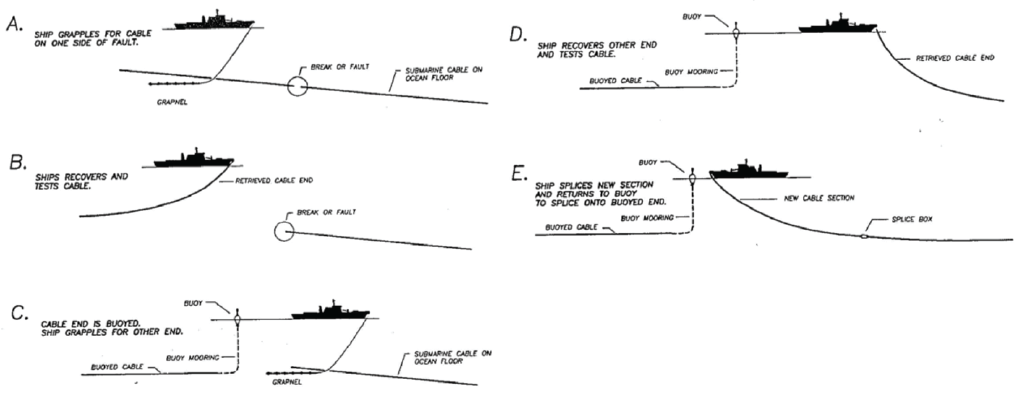
\includegraphics[width=14.17in]{figs/cable-repair-process} \caption{Ship operations for submarine cable repair. The ship runs a grapnel along the seafloor to catch the cable before the break, recovers and buoys one end of the cable, grapples and recovers the other, and splices a new section of repaired cable before laying it back onto the seafloor. Source: Tyco Electronics Subsea Communications, LLC}\label{fig:figSubmarineCableRepair}
\end{figure}

Although submarine cable locations are publicly accessible through
several publicly available datasets and electronic navigation charts, a
clear understanding of the areas where cable paths compete with
promising marine energy sites does not yet exist. By applying industry
advised setback distances from existing cables, we seek to minimize
conflict between this vital industry and the growing blue economy of
marine renewable energy.

\hypertarget{methods}{%
\section{Methods}\label{methods}}

\hypertarget{study-area-submarine-cables-depth-and-energy-data}{%
\subsection{Study Area, Submarine Cables, Depth and Energy
Data}\label{study-area-submarine-cables-depth-and-energy-data}}

The study area consisted of the US waters (Flanders Marine Institute
2016), i.e.~the 200 nm extent deemed the exclusive economic zone (EEZ).
We used the most comprehensive publicly available submarine cable
dataset ``NOAA Charted Submarine cables in the United States as of
December 2012'' available through MarineCadastre.gov.\footnote{MarineCadastre.gov
  cable metadata:
  \url{https://coast.noaa.gov/dataservices/Metadata/TransformMetadata?u=https://coast.noaa.gov/data/Documents/Metadata/harvest/MarineCadastre/NOAAChartedSubmarineCables.xml\&f=html}}
The contiguous US is further divided to yield the following analytical
territories: Alaska, Hawaii, West coast, East coast, Gulf of Mexico,
Puerto Rico, US Virgin Islands and Pacific Islands (Guam, Johnston
Atoll, N. Mariana Islands, Palmyra Atoll and Wake Island). The Gulf of
Mexico description based on the International Hydrographic Organization
(IHO) Sea Areas (VLIZ 2017) was used to separate the original Atlantic
US territory into East coast and Gulf of Mexico. To accommodate
territories overlapping the international dateline (Hawaii and Alaska),
all input and output products were shifted from {[}-180,180{]} to
{[}0,360{]} longitude space. The original 12 territories and cable
dataset are depicted on a map (Figure \ref{fig:mapCableTerritories})
before extraction of cables within the area of the 7 analyzed
territories (after lumping the Pacific Islands) within the US EEZ (Table
1).

\begin{figure}
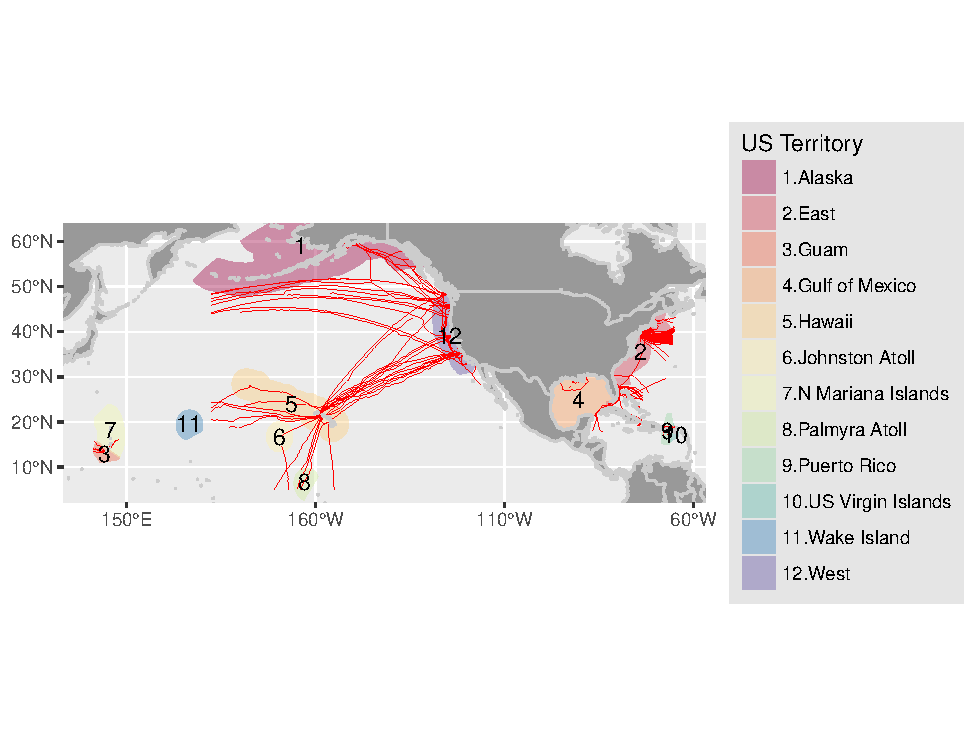
\includegraphics[width=6.5in]{figs/mapCableTerritories} \caption{Map of NOAA charted submarine cables (red lines) as of December 2012 within the exclusive economic zone (EEZ; 200 nm) overlapping with United States territories. Note throughout the rest of the report that some territories are grouped: Pacific Island territories (Guam, Johnston Atoll, N. Mariana Islands, Palmyra Atoll, Wake Island) and Atlantic Island territories (Puerto Rico, US Virgin Islands).}\label{fig:mapCableTerritories}
\end{figure}

Bathymetric depth, using the
\href{http://www.gebco.net/data_and_products/gridded_bathymetry_data/gebco_30_second_grid/}{GEBCO
30 arc-second grid}\footnote{GEBCO\_2014 Grid, version 20150318,
  www.gebco.net} (Weatherall et al. 2015), was used to extract the depth
of the cables and energy resource characterizations.

The marine renewable energy datasets from NREL are accessible online via
NREL's Wind Prospector\footnote{NREL Wind Prospector:
  \url{https://maps.nrel.gov/wind-prospector/}} and MHK Atlas\footnote{NREL
  MHK Atlas: \url{https://maps.nrel.gov/mhk-atlas}}. Tidal data were
modeled using the Regional Ocean Modeling System and calibrated with
available measurements of tidal current speed and water level surface in
terms of watts per square meter (W/m\textsuperscript{2}) (Haas et al.
2011). Wave data is based on a 51-month Wavewatch III hindcast database
developed by the National Oceanographic and Atmospheric Administration's
(NOAA's) National Centers for Environmental Prediction for estimation of
wave power density in terms of kilowatts per meter (kW/m) (Jacobson et
al. 2011). Wind data is for average offshore wind speed in meters per
second (m/s) at a 90 m hub height\footnote{Wind data for 90-meter
  offshore: \url{http://www.nrel.gov/gis/data_wind.html}} (Schwartz et
al. 2010).

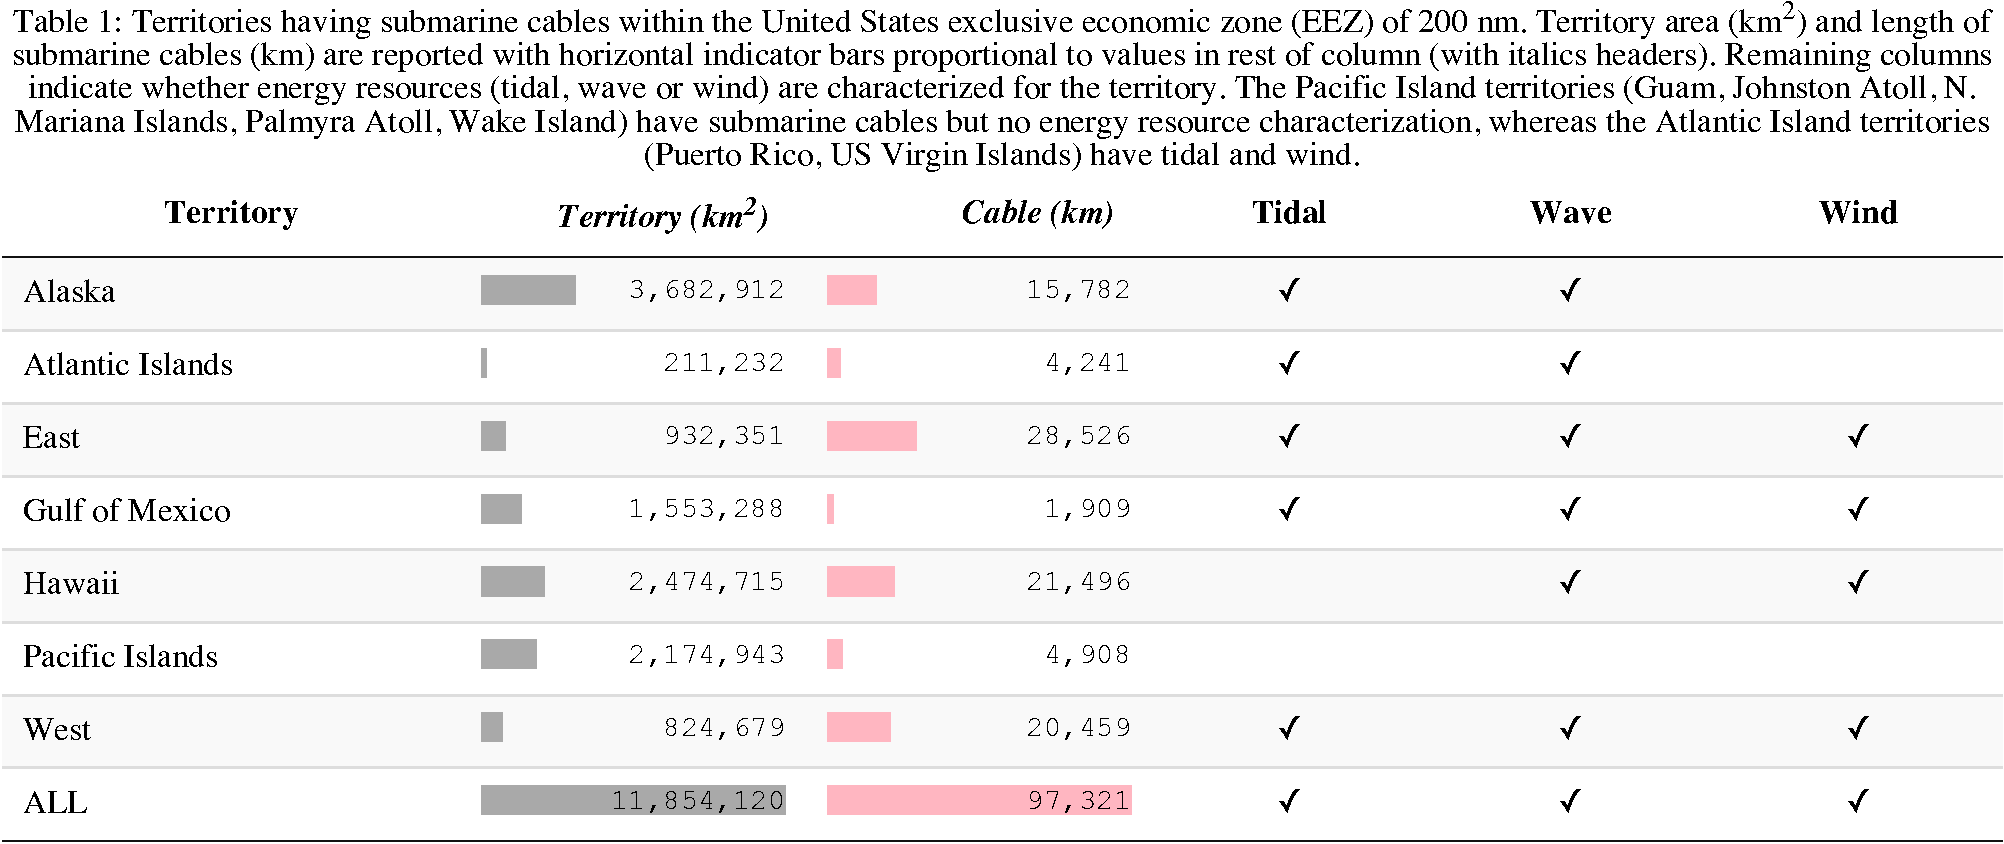
\includegraphics{report_files/figure-latex/tbl01Territories-1.pdf}

\hypertarget{submarine-cable-avoidance-zones}{%
\subsection{Submarine Cable Avoidance
Zones}\label{submarine-cable-avoidance-zones}}

The International Cable Protection Committee (ICPC)\footnote{International
  Cable Protection Committee (ICPC): \url{https://www.iscpc.org}} of the
North American Submarine Cable Association (NASCA)\footnote{North
  American Submarine Cable Association (NASCA):
  \url{https://www.n-a-s-c-a.org}} outlined recommended setback
distances (Communications Security, Reliability and Interoperability
Council IV 2014, 2016) for siting new offshore renewable wind energy
facilities and routing new cables.

\begin{itemize}
\item
  \textbf{New Facilities}: the maximum of 500 m or twice the bottom
  depth (2z), per ICPC Recommendation 13 No.~2 (Communications Security,
  Reliability and Interoperability Council IV 2014). For depths
  \textless{}= 250 m, a 500 m buffer from the cables applies and for
  depths \textgreater{} 250 m, 2 * depth is to be used. This product is
  referred to as the ``facilities (2z)'' product throughout this report.
\item
  \textbf{New Cables}: the maximum of 500 m or thrice the bottom depth
  (3z), per ICPC Recommendation 2 No.~10 (Communications Security,
  Reliability and Interoperability Council IV 2014). So for depths
  \textless{}= 250 m, a 500 m buffer from the cables applies and for
  depths \textgreater{} 250 m, 3 * depth is to be used. This product is
  referred to as the ``cables (3z)'' product throughout this report.
\end{itemize}

\hypertarget{depth-varying-cable-buffer}{%
\subsection{Depth-Varying Cable
Buffer}\label{depth-varying-cable-buffer}}

A depth-varying buffer from existing submarine cables for new facilities
(2z) and cables (3z) was calculated by intersecting depth with cables
and buffering the cable segment by the depth multiplier. Depth from the
GEBCO grid was reclassed into 100 m increments starting with 250 m to
apply a 500 m minimum for the 2z and 3z products, and converted to
polygons for intersecting with the cable linear features. A custom
Albers Equal Area Conic projection based on 1/6th the extent\footnote{The
  ``one-sixth rule'' for Albers Equal Area Conic projection:
  \url{http://desktop.arcgis.com/en/arcmap/latest/map/projections/albers-equal-area-conic.htm\#GUID-2158C4F9-F197-458E-94F0-84933C1BE6B7}}
of each territory was individually applied to minimize spatial
distortion when buffering.

\hypertarget{reproducible-code}{%
\subsection{Reproducible Code}\label{reproducible-code}}

In the spirit of reproducible research (Lowndes et al. 2017; Madeyski
and Kitchenham 2015), all analytical code to generate outputs, including
this data driven report, are available in a publicly accessible online
repository: \url{http://github.com/ecoquants/nrel-cables}. Here are
particularly noteworthy files:

\begin{itemize}
\tightlist
\item
  \texttt{data/}

  \begin{itemize}
  \tightlist
  \item
    \href{https://github.com/ecoquants/nrel-cables/blob/master/data/lns_d1x.geojson}{\texttt{lns\_d1x.geojson}}:
    lines of submarine cables segmented at 100 m increments with depth
    value for buffering, i.e.~minimum 500 m and depth (z) for
    multiplying by 2 (2z) or 3 (3z).
  \item
    \href{https://github.com/ecoquants/nrel-cables/blob/master/data/buf_2xdepth_incr100m.geojson}{\texttt{buf\_2xdepth\_incr100m.geojson}}:
    polygons for siting new facilities buffered from existing submarine
    cables at twice the depth (2z), minimum 500 m.
  \item
    \href{https://github.com/ecoquants/nrel-cables/blob/master/data/buf_3xdepth_incr100m.geojson}{\texttt{buf\_3xdepth\_incr100m.geojson}}:
    polygons for siting new cables buffered from existing submarine
    cables at three times the depth (3z), minimum 500 m.
  \end{itemize}
\item
  \texttt{docs/}

  \begin{itemize}
  \tightlist
  \item
    \href{https://github.com/ecoquants/nrel-cables/blob/master/docs/packages_vars.R}{\texttt{packages\_vars.R}}:
    R code with variables and packages used across analysis
    (\texttt{create\_cable-buffer.R}, \texttt{extract\_cable-energy.R})
    and reporting (\texttt{report.Rmd})
  \item
    \href{https://github.com/ecoquants/nrel-cables/blob/master/docs/create_cable-buffer.R}{\texttt{create\_cable-buffer.R}}:
    R code to generate cable buffers at 100 m depth increments.
  \item
    \href{https://github.com/ecoquants/nrel-cables/blob/master/docs/extract_cable-energy.R}{\texttt{extract\_cable-energy.R}}:
    R code to extract renewable energy for cabled territories.
  \item
    \href{https://github.com/ecoquants/nrel-cables/blob/master/docs/report.Rmd}{\texttt{report.Rmd}}:
    R markdown document for reproducible, data-driven generation of
    various report output file formats (\texttt{report.pdf},
    \texttt{report.docx}, \texttt{report.html})
  \end{itemize}
\end{itemize}

\hypertarget{results}{%
\section{Results}\label{results}}

\hypertarget{cable-buffer}{%
\subsection{Cable Buffer}\label{cable-buffer}}

Of the original 230,835 km of cable in the ``NOAA Charted Submarine
cables in the United States as of December 2012'' dataset (Figure
\ref{fig:mapCableTerritories}), 97,321 km fell within the 200 nm of the
US exclusive economic zone (EEZ), which was analyzed across 12
territories that overlapped with the cables (Figure
\ref{fig:mapCableTerritories}). The cable buffer area ranged from
29.35\% (242,031 km\textsuperscript{2} {[}3z{]} of 824,679
km\textsuperscript{2} total) in the West owing to many cables present
and the steep continental shelf, to virtually nill 0.39\% (6,133
km\textsuperscript{2} {[}2z{]} of 1,553,288 km\textsuperscript{2} total)
in Gulf of Mexico (Table 2).

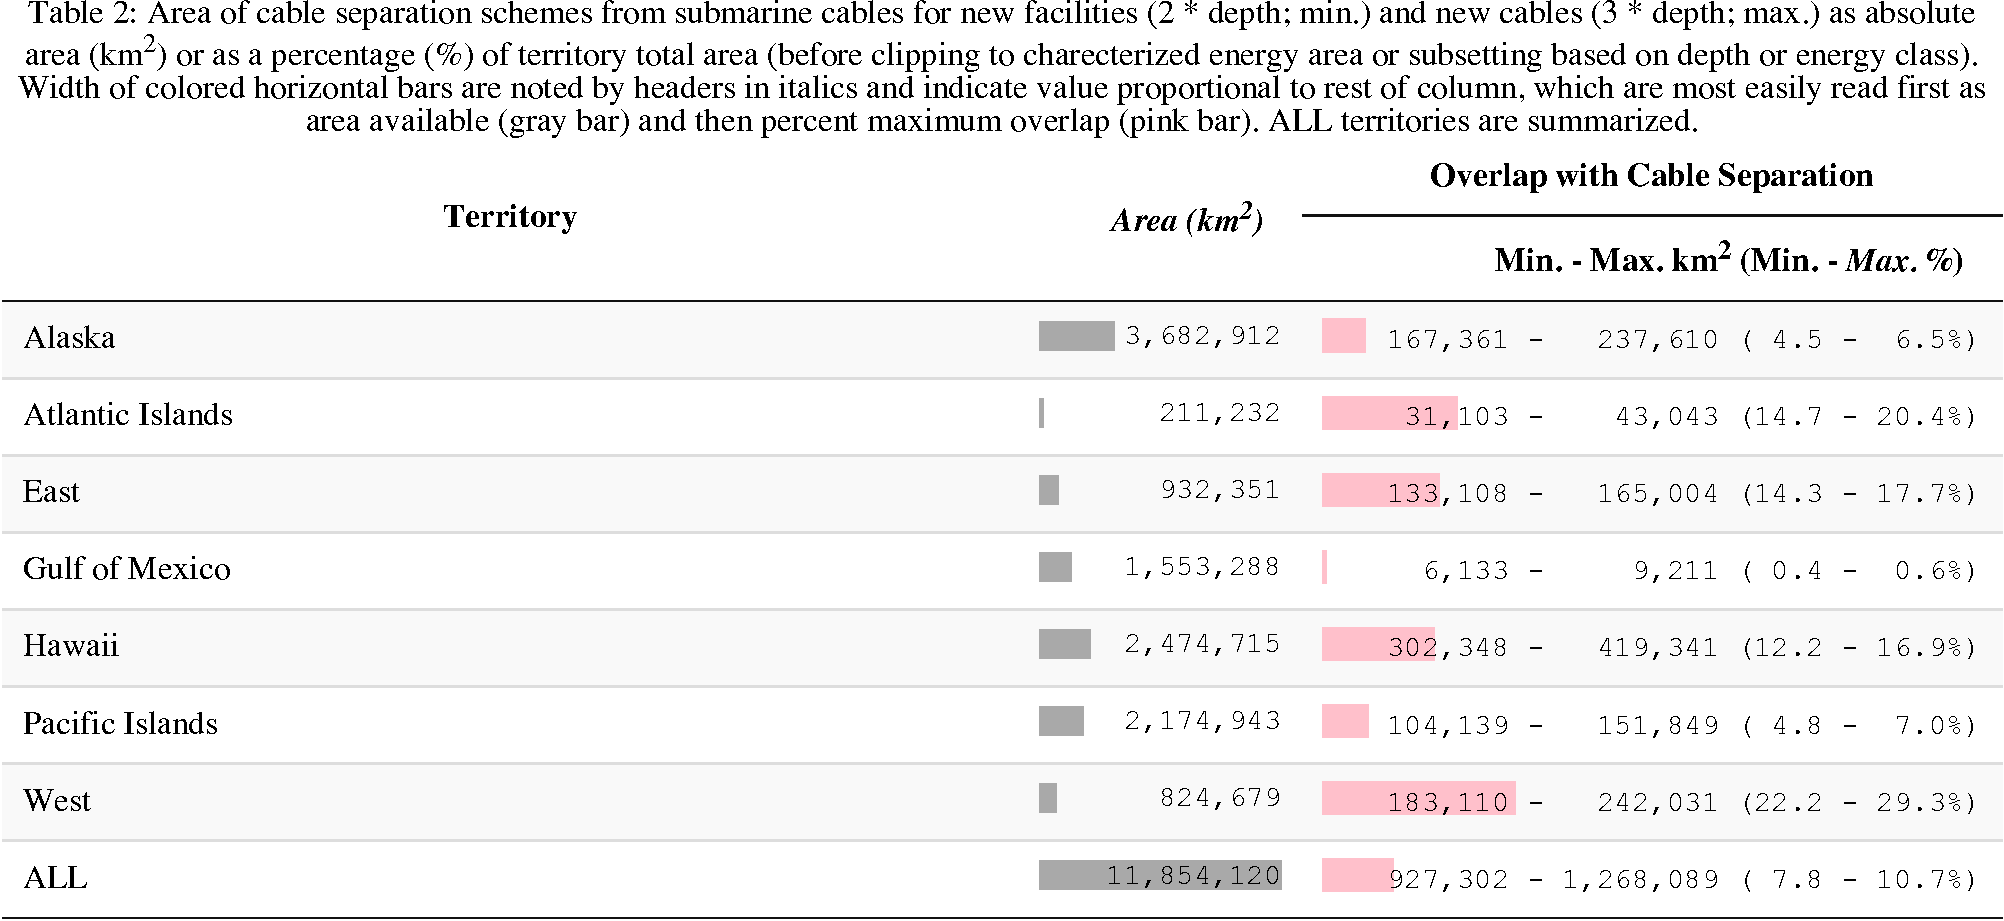
\includegraphics{report_files/figure-latex/tbl02CableBufferTerritories-1.pdf}

\hypertarget{overlap-of-cable-buffer-with-renewable-energy}{%
\subsection{Overlap of Cable Buffer with Renewable
Energy}\label{overlap-of-cable-buffer-with-renewable-energy}}

Overlap of cable buffers with marine renewable energy was assessed for
tidal (Haas et al. 2011), wave (Jacobson et al. 2011) and wind (Schwartz
et al. 2010) energy based on energy resource characterizations available
through the National Renewable Energy Lab (NREL) Wind
Prospector\footnote{NREL Wind Prospector:
  \url{https://maps.nrel.gov/wind-prospector/}} or MHK Atlas\footnote{NREL
  MHK Atlas: \url{https://maps.nrel.gov/mhk-atlas}}. Assessment of
overlap with the advised separation schemes and energy resource was
limited to maximum depths based on current assessment of technology
limitations: \textless{} 100 m for tidal (Haas et al. 2011), \textless{}
200 m for wave (Jacobson et al. 2011), \textless{} 1,000 m for wind
(Musial et al. 2016). The lowest energy classes were also dropped from
the assessment (tidal: \textgreater{} 500 \(W/m^2\), wave:
\textgreater{} 10 \(kW/m\), wind: \textgreater{} 7 \(m/s\)) viable for
energy development.

Total area of viable tidal resource (1,671 \(km^2\)) is orders of
magnitude less than wave (378,908 \(km^2\)) or wind (462,613 \(km^2\))
owing to requirements for channelized bathymetry (Table 3). Nationally,
tidal energy has up to 3.8\% overlap, wave 0.9\% and wind 4\% (Table 3),
so conflict between viable marine renewable energy resource and existing
submarine cables is generally minimal. However a small fraction of
viable resource areas in high energy areas is notable. For instance, for
the small area (207 \(km^2\)) of highest wind speeds (11-12 m/s)
occurring only in Hawaii overlap is up to 37.9\% (Table 6). The lowest
tidal energy class (500 - 1,000 \(W/m^2\)) in the West region (11
\(km^2\)), largely around Puget Sound, has 31.5\% overlap (Table 4).

Viable tidal resource (Table 3) have up to 4.7\% overlap for the lowest
energy class (500 - 1,000 \(W/m^2\)) with only 2.3\% and 0.9\% overlap
at higher power classes 1,000 - 1,500 and \textgreater{} 1,500 \(W/m^2\)
respectively. Wave energy at either depth bin of 0 - 100 or 100 - 200 m
is very low with at most 2\% overlap for the lower energy class (10-20
\(kW/m\)) at depths 100 - 200 m. The most abundant viable wind in
shallow depth (0 - 100 m) and lower energy (7 - 8 and 8 - 9 \(m/s\))
overlaps at most 3.1\%, but overlaps more at higher speeds (9.6\% at 9 -
10 \(m/s\)) and in deeper waters (7.8\% and 10.5\% at 7 - 8 and 8 - 9
\(m/s\) respectively in depths 200 - 1,000 m). Small areas at the
highest wind speeds \textgreater{} 10 \(m/s\) overlap up to 42.1\% for
the deepest bin (200 - 1,000 m) and highest wind speeds (11 - 12
\(m/s\)).

Energy resources are unevenly distributed across territories. Tidal
power (Table 4) is most abundant in Alaska (691 \(km^2\) at 500 - 1,000
\(W/m^2\)), the East (390 \(km^2\) at 500 - 1,000 \(W/m^2\)) and the
West (46 \(km^2\) at 500 - 1,000 \(W/m^2\)), which is where overlap with
cable buffers is most significant (23.4 - 31.5\%) such as around Port
Townsend, WA (Figure \ref{fig:mapTideWest}). Wave energy (Table 5) is
most abundant in the Pacific territories having the most exposure to
storm activity across the largest ocean. Alaska has the most abundant
energy across all viable energy classes. Wind speeds (Table 6) in excess
of 9 \(m/s\) are not found in the Gulf of Mexico and limited to the
offshore New England area of the East (Figure \ref{fig:mapWindEast}),
offshore areas of California and Oregon in the West (Figure
\ref{fig:mapWindEast}) and dispersed locations in Hawaii (Figure
\ref{fig:mapWindEast}).

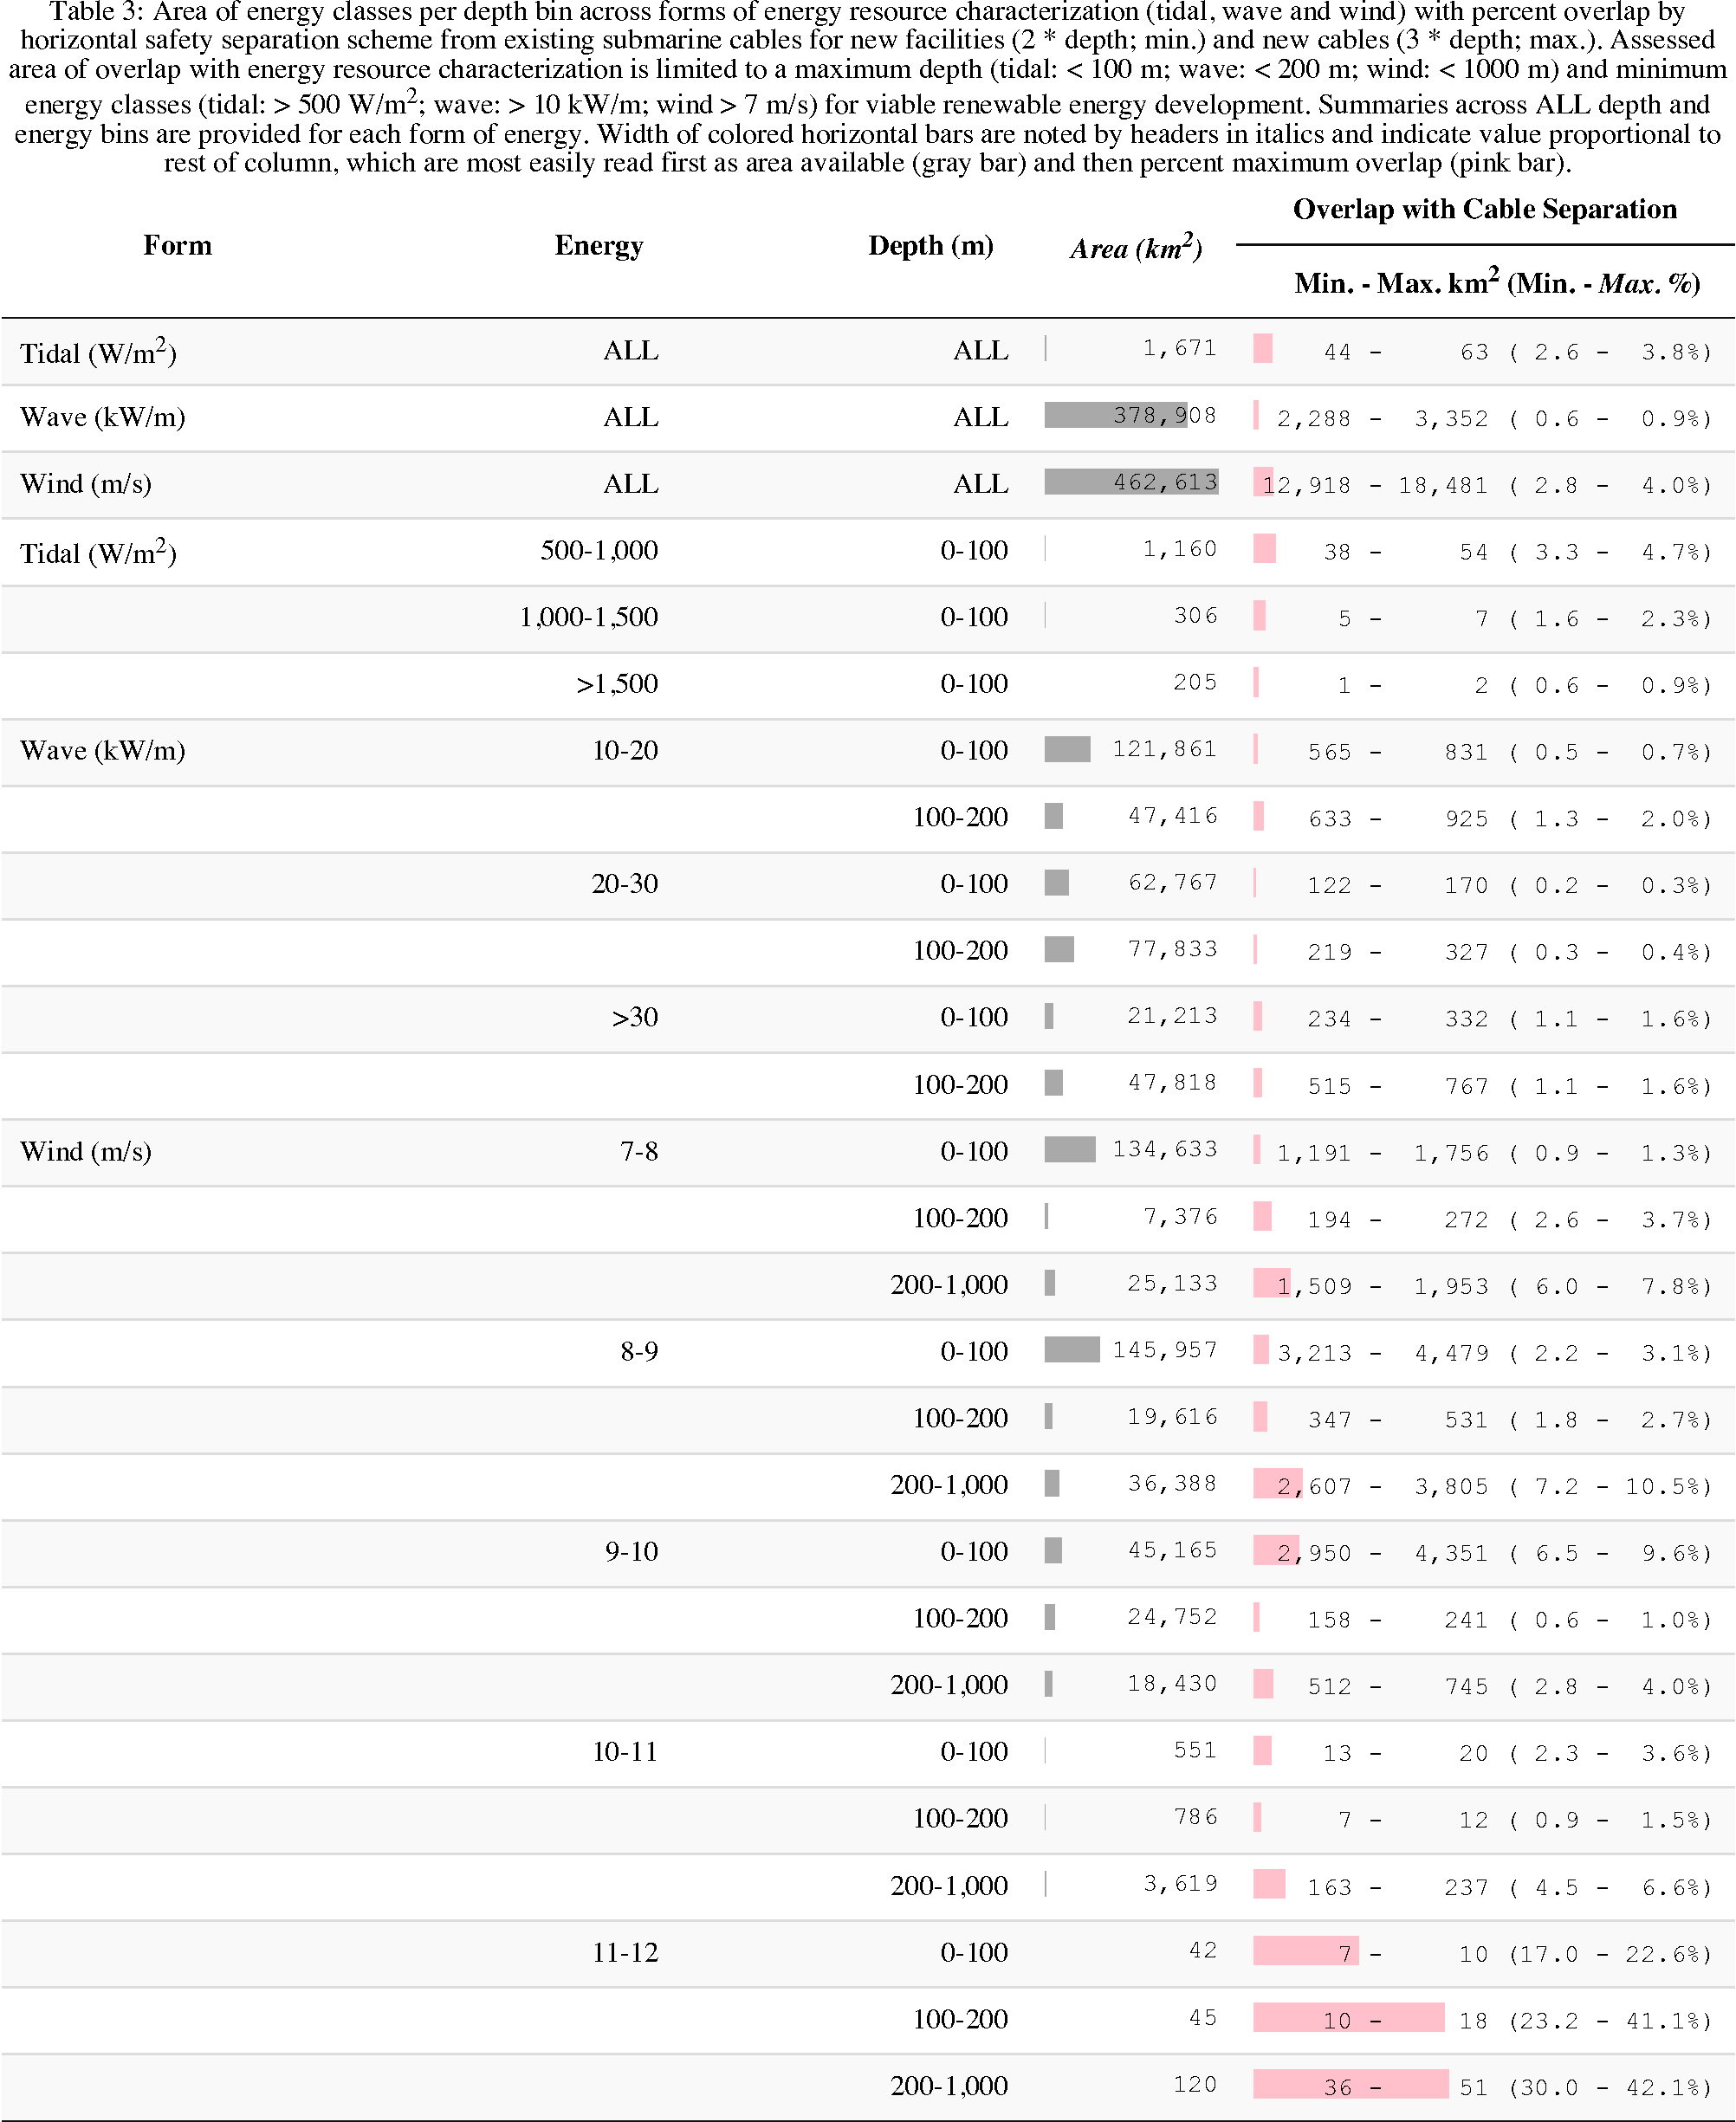
\includegraphics{report_files/figure-latex/tbl03Energy-1.pdf}

\hypertarget{tidal}{%
\subsubsection{Tidal}\label{tidal}}

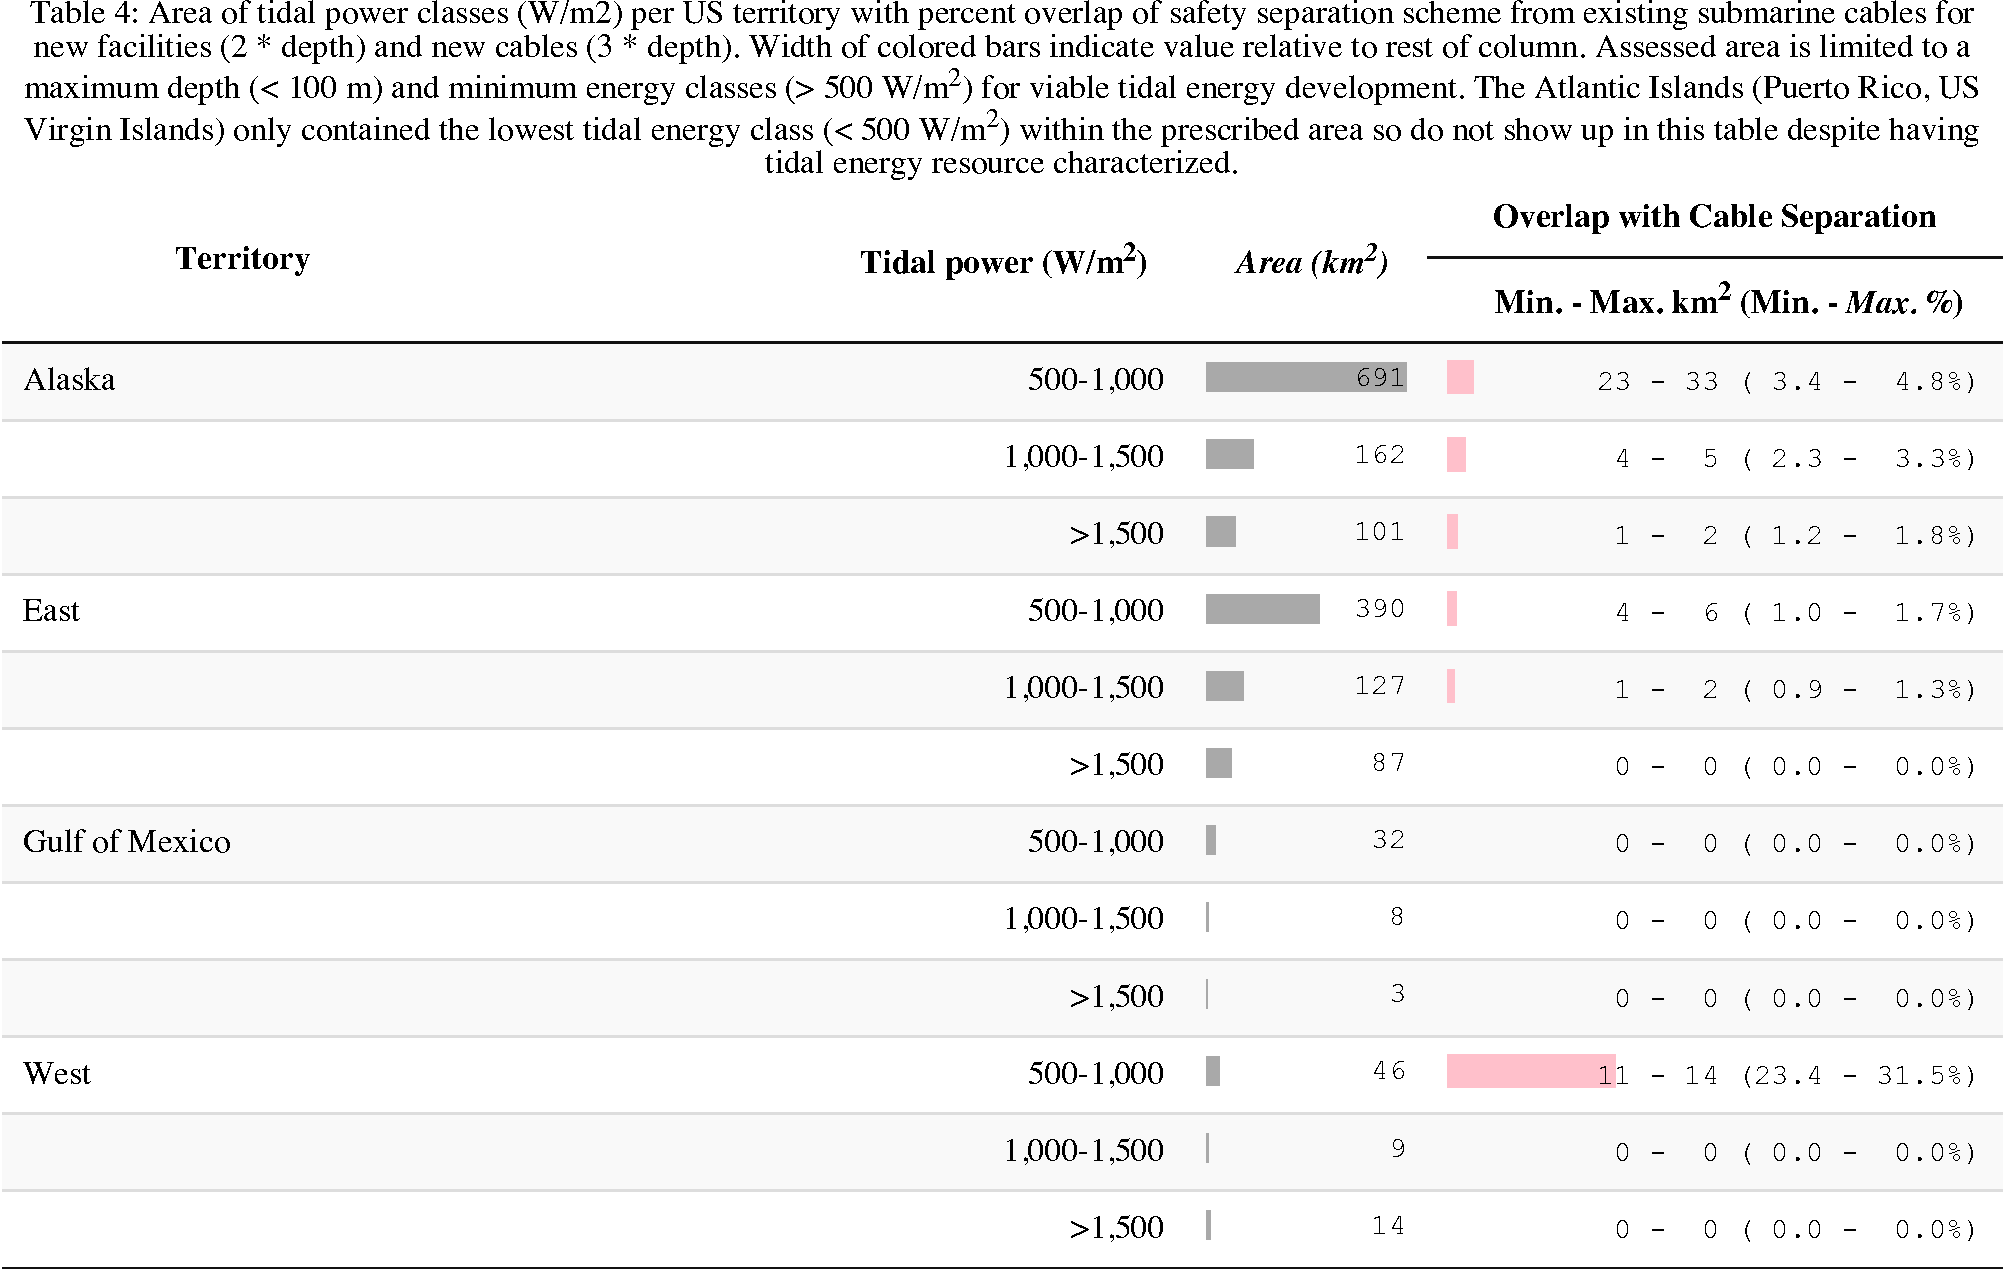
\includegraphics{report_files/figure-latex/tbl04Tide-1.pdf}

\hypertarget{wave}{%
\subsubsection{Wave}\label{wave}}

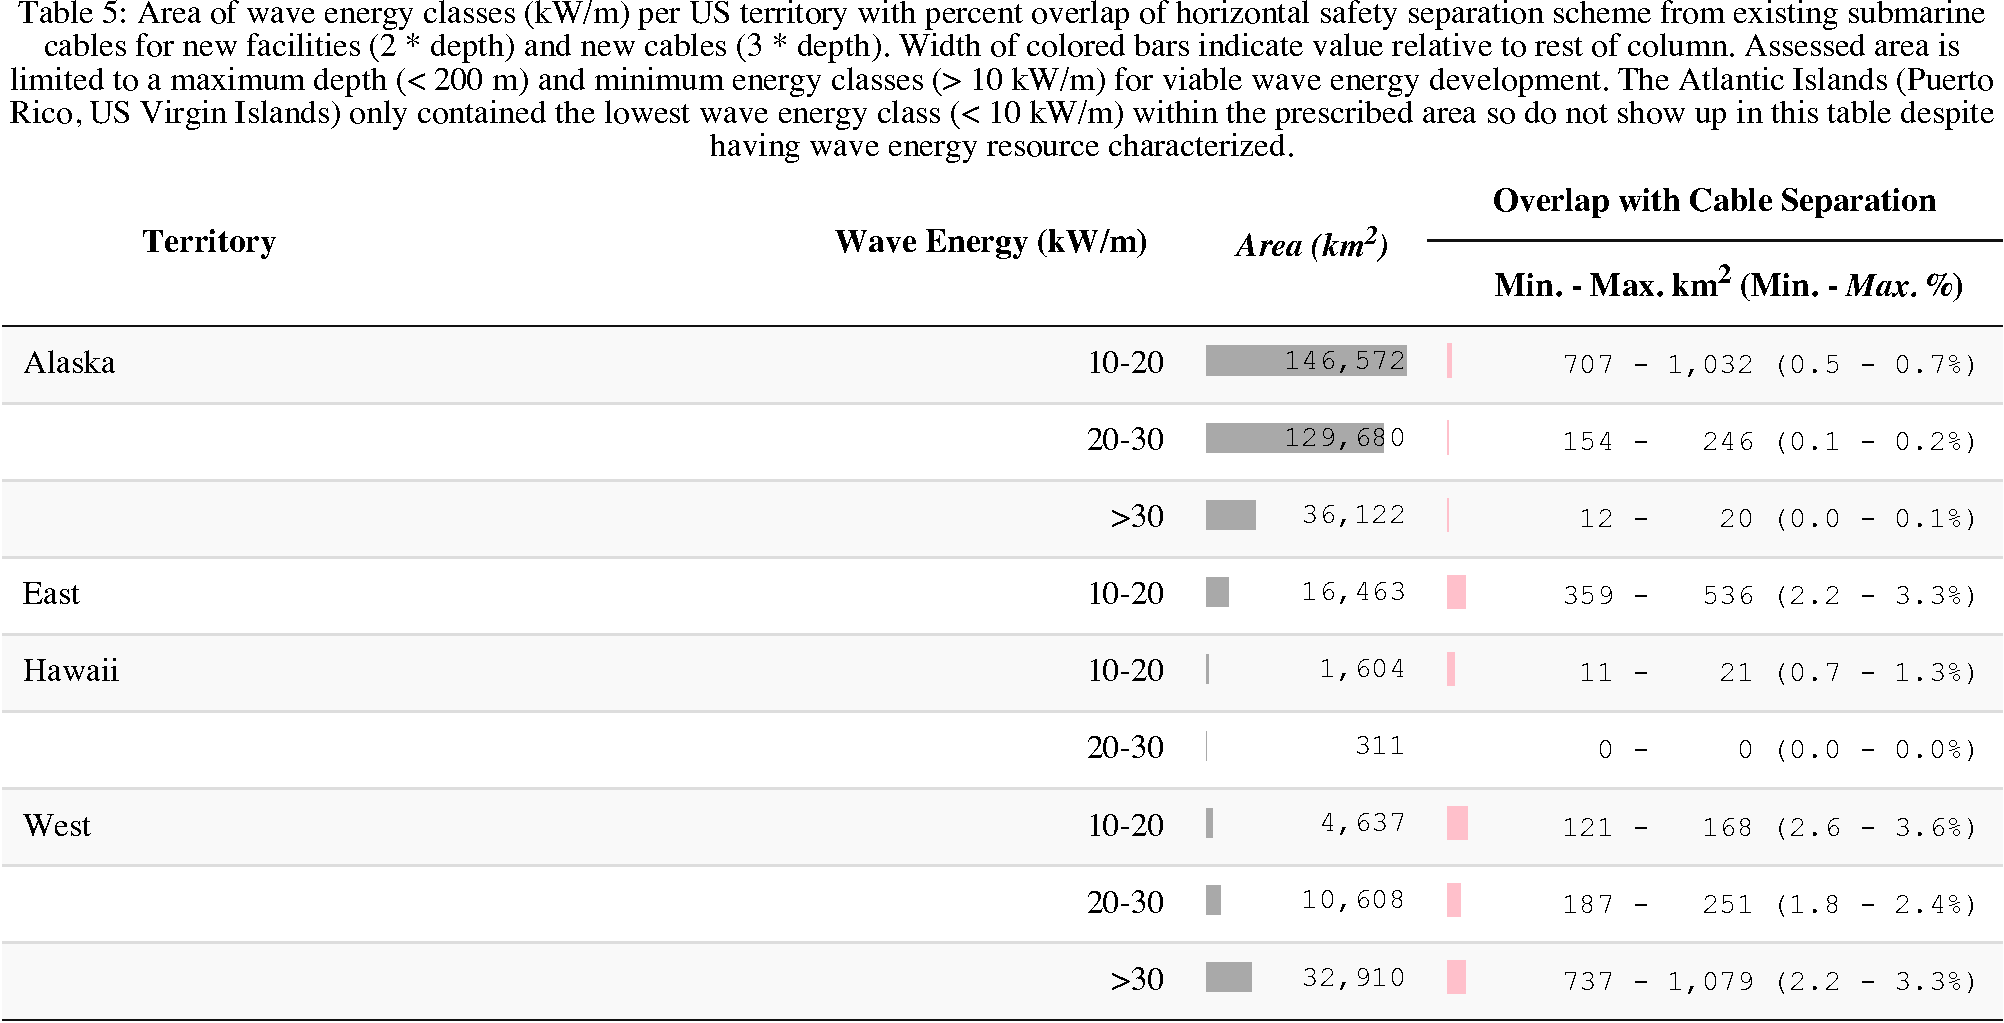
\includegraphics{report_files/figure-latex/tbl05Wave-1.pdf}

\hypertarget{wind}{%
\subsubsection{Wind}\label{wind}}

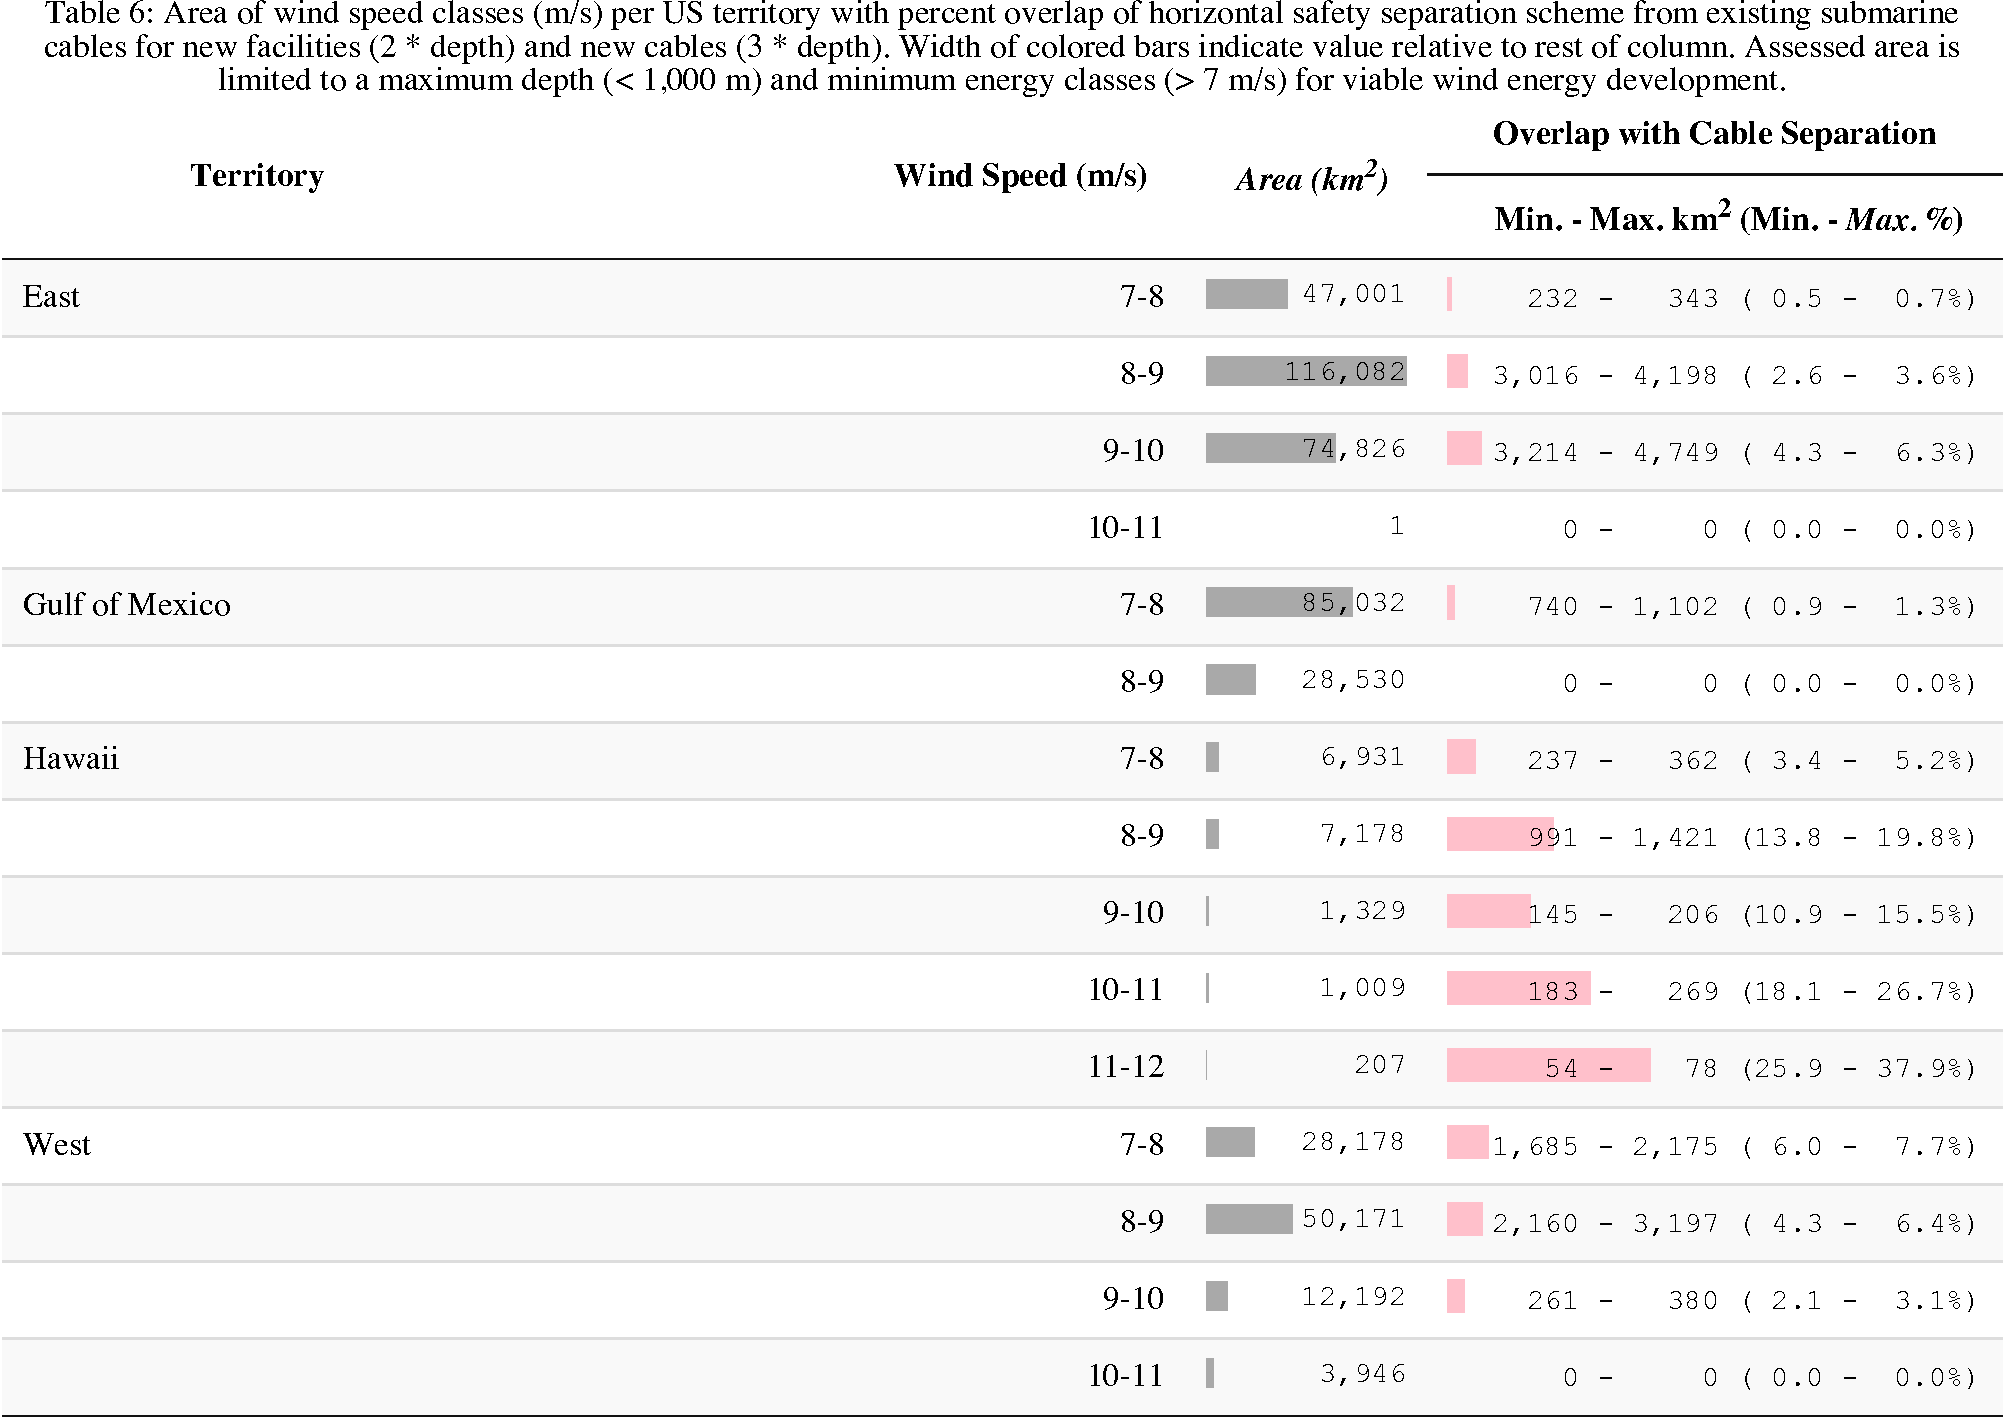
\includegraphics{report_files/figure-latex/tbl06Wind-1.pdf}

\hypertarget{discussion}{%
\section{Discussion}\label{discussion}}

Besides the \href{http://marinecadastre.gov}{Marine Cadastre} national
marine spatial planning effort coordinated by NOAA and BOEM, other ocean
regional planning efforts recognize submarine cables in their data
catalogs: \href{http://midatlanticocean.org}{Mid-Atlantic Regional Ocean
Council (MARCO)} portal (New York, New Jersey, Delaware, Maryland and
Virginia); \href{http://northeastoceancouncil.org/}{Northeast Regional
Ocean Council (NROC)} portal (Maine, New Hampshire, Vermont,
Massachusetts, Rhode Island, and Connecticut);
\href{http://southatlanticalliance.org/}{Governors' South Atlantic
Alliance (GSAA)} portal (North Carolina, South Carolina, Georgia and
Florida); \href{http://www.gulfofmexicoalliance.org/}{Gulf of Mexico
Alliance} portal (Florida, Alabama, Mississippi, Louisiana and Texas);
and \href{http://www.westcoastoceans.org/}{West Coast Ocean Partnership}
(Washington, Oregon and California).

Although the US currently only has one marine renewable energy facility
in full production at Block Island NJ, many more are in pilot and
proposal phases\footnote{BOEM Renewable Energy Programs state
  activities:
  \url{https://www.boem.gov/Renewable-Energy-State-Activities/}} with
much future potential (Beiter et al. 2017; Lehmann et al. 2017; Uihlein
and Magagna 2016). The Virginia Wind Energy Area (WEA) offshore from
Virginia Beach currently has five proposed/ongoing offshore wind related
activities with some potential for conflict given three submarine cables
ready for service in the near future, discoverable via
\href{http://submarinecablemap.com}{SubmarineCableMap.com}: MAREA (Q1
2018), Midgardsormen (Q2 2019), BRUSA (Q2 2018). In New York the
Interior Department auctioned nearly 80,000 acres offshore for
commercial wind energy development in December, 2016. New Jersey has 2
renewable energy leases signed by BOEM as of February, 2016. In
Massachusetts, BOEM approved the site assessment plan for a lease with
Bay State Wind in June of 2017 and is in process with another offshore
lease between Statoil Wind and PNE Wind with bids received in January,
2017. In Rhode Island, besides the existing Block Island wind facility
in production, BOEM is reviewing a site assessment plan for the North
Lease Area recieved from Deepwater Wind April of 2016. In Delaware on
December of 2016 BOEM approved the assignment of an offshore wind lease
to GSOE I. In Oregon, Oregon State University's Northwest National
Marine Renewable Energy Center is in the permitting phase to develop the
South Energy Test Site (SETS) facility for testing wave energy
converters (WECs). In California, a competitive bidding process is
underway between Trident Winds and Statoil Wind for an offshore area
near Morro Bay. In Hawaii, BOEM is in the area identification stage of
the leasing process for two call areas north and south of Oahu.

\hypertarget{conclusion}{%
\section{Conclusion}\label{conclusion}}

Marine renewable energy promises to be a large expanding section of the
``blue economy'' that rides on the wave of the ``green economy'' for
creating new jobs and reducing dependence on foreign energy sources. In
fact wind turbine service technician is the single fastest growing
occupation in America with 25,000 new jobs added last year to now be at
over 100,000 workers nationally (Bureau of Labor Statistics
2017\footnote{Bureau of Labor Statistics:
  \url{https://www.bls.gov/ooh/fastest-growing.htm}}). Decreasing
dependency on foreign oil is critical to preventing future energy
calamities such as the 1973 oil crisis in which an oil embargo to the
U.S. was placed by the Organization of Arab Petroleum Exporting
Countries (OAPEC) due to political actions related to supporting Israel.
Furthermore, given the climate change impacts of fossil fuel energy
production (Pachauri et al. 2015), development of clean renewable energy
alternatives are imperative for the sustainable future of the United
States and rest of the planet.

These energy sources however vary widely in geographic and temporal
availability and may compete with other uses. The submarine cable
industry provides critical power and telecommunication services, such
that safe operation and maintenance must be heeded as marine renewable
energy sources are developed (Communications Security, Reliability and
Interoperability Council IV 2014, 2016). The submarine cable safety
avoidance zones created and evaluated through this report are products
intended to minimize conflict at the planning stage between these
competing uses.

The proposed avoidance areas for submarine cables should be deemed
advisory. Overlap with the new facility (3z) or cable (2z) buffers
around existing submarine cables does not nullify the possibility of
renewable energy development there. Rather, it should alert the
developer to negotiate reasonable terms with the cable operator via
contacting the cable industry, such as the North American Submarine
Cable Association\footnote{North American Submarine Cable Association
  (NASCA): \url{https://www.n-a-s-c-a.org}} or the International Cable
Protection Committee\footnote{International Cable Protection Committee
  (ICPC): \url{https://www.iscpc.org}}. These avoidance zones are
advised according to traditional methods of submarine cable repair
involving grappling of the submarine cable and buoying to the surface
for repair, hence allowance for sway of boat as a function of depth. In
future, use of more sophisticated remotely operated vehicles may narrow
safe operating distances. These avoidance areas are limited to the most
recent submarine cable data. Any planning for marine renewable energy
should consult the latest electronic navigation charts and contact the
cable industry for confirmation.

Overlap between existing submarine cables and viable marine renewable
energy sources is generally minimal (maximum 3.8\% for tidal, 0.9\% for
wave and 4.0\% for wind; Table 3) meaning the two industries are
generally compatible into the future. Specific high energy areas already
noted, such as Puget Sound for tidal, Oregon for wave, and Oahu for
wind, do exist and may inevitably conflict with future plans
(e.g.~planned cables and wind energy areas in Virginia Beach), however
reasonable terms for operation and maintenance are negotiable. This new
spatial separation scheme from existing submarine cables serves to alert
developers so such negotiations can be an early part of the planning
process.

\newpage

\hypertarget{appendix-appendix}{%
\appendix}


\hypertarget{maps-by-us-territory-of-cable-buffer-and-renewable-energy}{%
\section{Maps by US Territory of Cable Buffer and Renewable
Energy}\label{maps-by-us-territory-of-cable-buffer-and-renewable-energy}}

\hypertarget{tide}{%
\subsection{Tide}\label{tide}}

\hypertarget{alaska}{%
\subsubsection{Alaska}\label{alaska}}

\begin{figure}
\centering
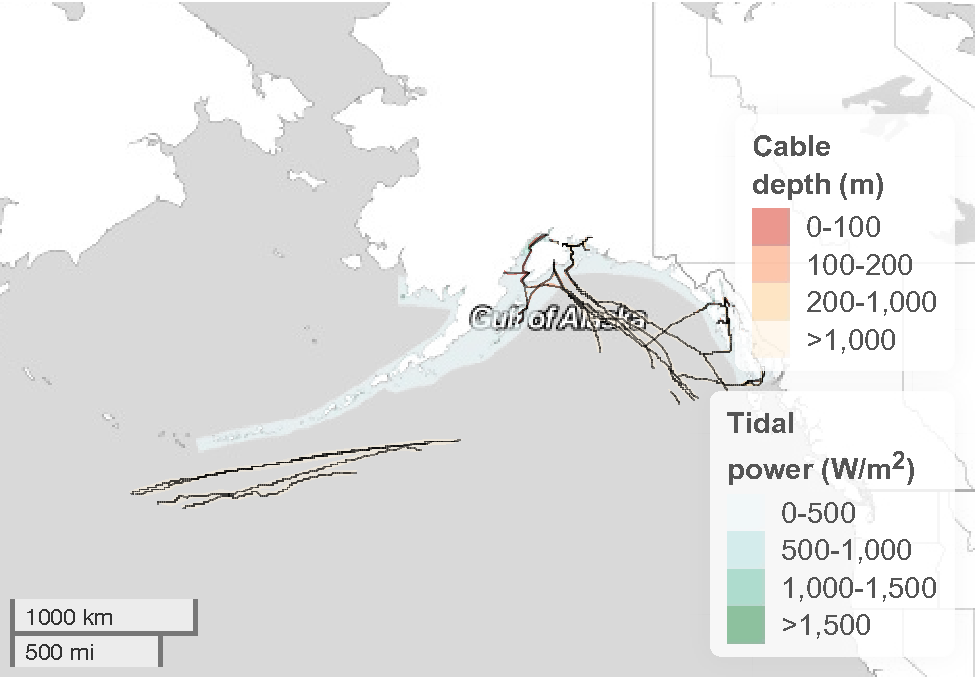
\includegraphics{report_files/figure-latex/mapTideAlaska-1.pdf}
\caption{\label{fig:mapTideAlaska}Map of tidal power (\(W/m^2\)) in Alaska
with submarine cables (black lines) and advisory buffers colored by
bottom depth. The buffers are plotted with transparency so the inner
more opaque band represents the advised horizontal separation scheme for
new facilities (2 * depth) and outer less opaque band the scheme for new
cables (3 * depth). At large scales this detail is not visible.
Alternatively, you can zoom and pan interactively on these layers at
\url{http://ecoquants.github.io/nrel-cables/maps.html}.}
\end{figure}

\hypertarget{east}{%
\subsubsection{East}\label{east}}

\begin{figure}
\centering
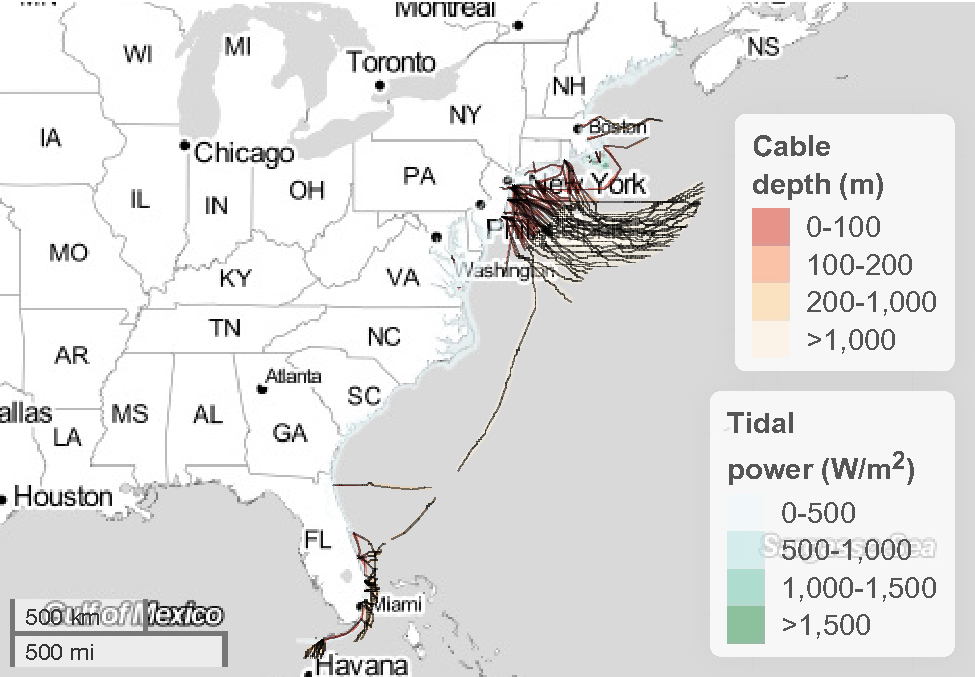
\includegraphics{report_files/figure-latex/mapTideEast-1.pdf}
\caption{\label{fig:mapTideEast}Map of tidal power (\(W/m^2\)) in the East
with submarine cables (black lines) and advisory buffers colored by
bottom depth. The buffers are plotted with transparency so the inner
more opaque band represents the advised horizontal separation scheme for
new facilities (2 * depth) and outer less opaque band the scheme for new
cables (3 * depth). At large scales this detail is not visible.
Alternatively, you can zoom and pan interactively on these layers at
\url{http://ecoquants.github.io/nrel-cables/maps.html}.}
\end{figure}

\hypertarget{gulf-of-mexico}{%
\subsubsection{Gulf of Mexico}\label{gulf-of-mexico}}

\begin{figure}
\centering
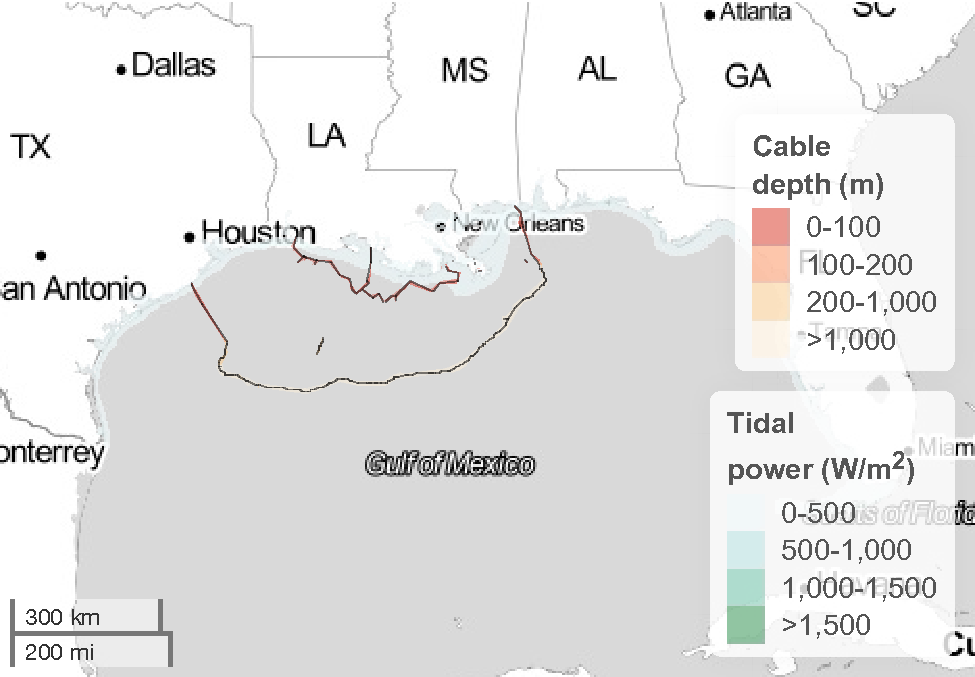
\includegraphics{report_files/figure-latex/mapTideGulfofMexico-1.pdf}
\caption{\label{fig:mapTideGulfofMexico}Map of tidal power (\(W/m^2\)) in
the Gulf of Mexico with submarine cables (black lines) and advisory
buffers colored by bottom depth. The buffers are plotted with
transparency so the inner more opaque band represents the advised
horizontal separation scheme for new facilities (2 * depth) and outer
less opaque band the scheme for new cables (3 * depth). At large scales
this detail is not visible. Alternatively, you can zoom and pan
interactively on these layers at
\url{http://ecoquants.github.io/nrel-cables/maps.html}.}
\end{figure}

\hypertarget{puerto-rico}{%
\subsubsection{Puerto Rico}\label{puerto-rico}}

\begin{figure}
\centering
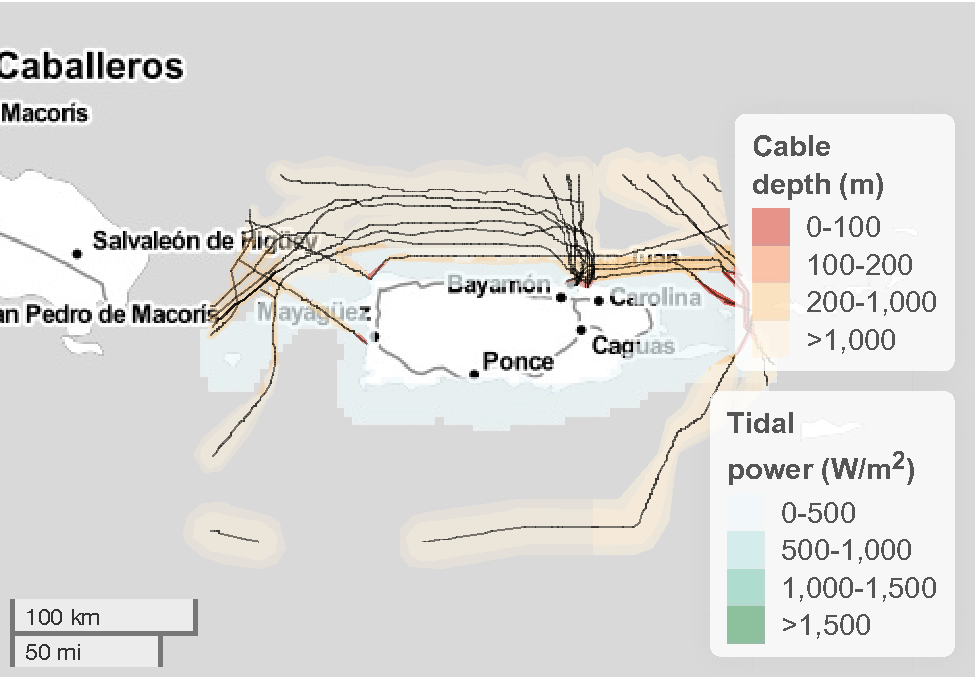
\includegraphics{report_files/figure-latex/mapTidePuertoRico-1.pdf}
\caption{\label{fig:mapTidePuertoRico}Map of tidal power (\(W/m^2\)) in
Puerto Rico with submarine cables (black lines) and advisory buffers
colored by bottom depth. The buffers are plotted with transparency so
the inner more opaque band represents the advised horizontal separation
scheme for new facilities (2 * depth) and outer less opaque band the
scheme for new cables (3 * depth). At large scales this detail is not
visible. Alternatively, you can zoom and pan interactively on these
layers at \url{http://ecoquants.github.io/nrel-cables/maps.html}.}
\end{figure}

\hypertarget{us-virgin-islands}{%
\subsubsection{US Virgin Islands}\label{us-virgin-islands}}

\begin{figure}
\centering
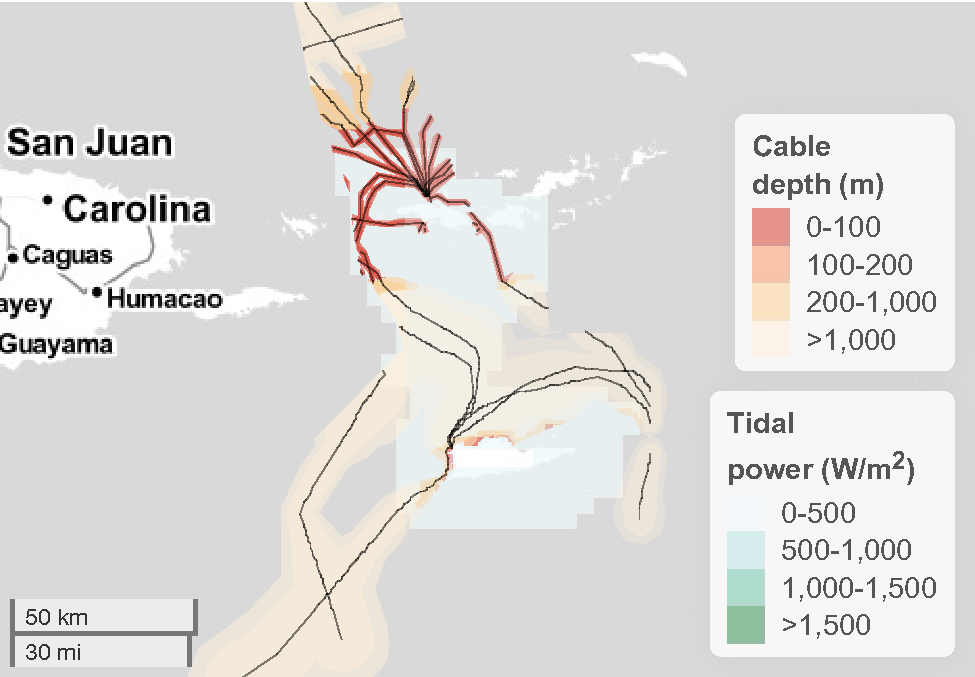
\includegraphics{report_files/figure-latex/mapTideUSVirginIslands-1.pdf}
\caption{\label{fig:mapTideUSVirginIslands}Map of tidal power (\(W/m^2\)) in
the US Virgin Islands with submarine cables (black lines) and advisory
buffers colored by bottom depth. The buffers are plotted with
transparency so the inner more opaque band represents the advised
horizontal separation scheme for new facilities (2 * depth) and outer
less opaque band the scheme for new cables (3 * depth). At large scales
this detail is not visible. Alternatively, you can zoom and pan
interactively on these layers at
\url{http://ecoquants.github.io/nrel-cables/maps.html}.}
\end{figure}

\hypertarget{west}{%
\subsubsection{West}\label{west}}

\begin{figure}
\centering
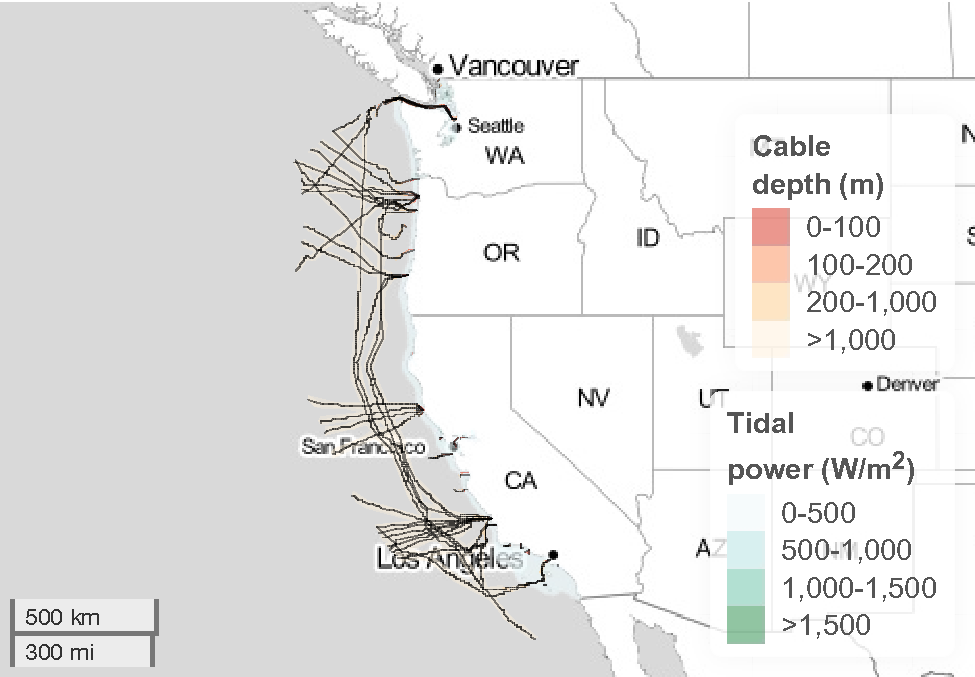
\includegraphics{report_files/figure-latex/mapTideWest-1.pdf}
\caption{\label{fig:mapTideWest}Map of tidal power (\(W/m^2\)) in the West
with submarine cables (black lines) and advisory buffers colored by
bottom depth. The buffers are plotted with transparency so the inner
more opaque band represents the advised horizontal separation scheme for
new facilities (2 * depth) and outer less opaque band the scheme for new
cables (3 * depth). At large scales this detail is not visible.
Alternatively, you can zoom and pan interactively on these layers at
\url{http://ecoquants.github.io/nrel-cables/maps.html}.}
\end{figure}

\hypertarget{wave-1}{%
\subsection{Wave}\label{wave-1}}

\hypertarget{alaska-1}{%
\subsubsection{Alaska}\label{alaska-1}}

\begin{figure}
\centering
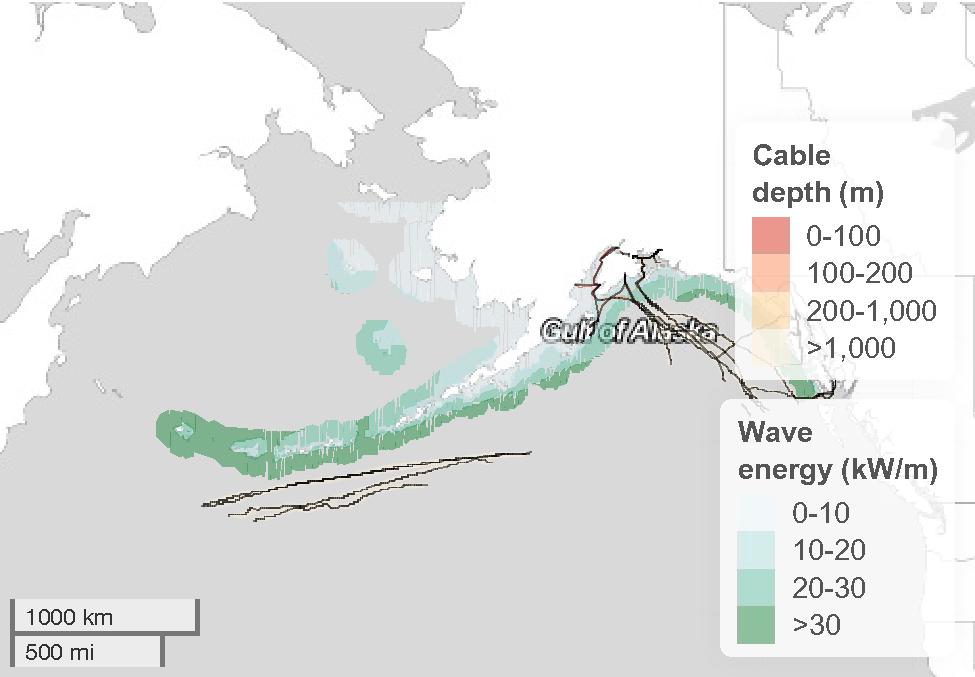
\includegraphics{report_files/figure-latex/mapWaveAlaska-1.pdf}
\caption{\label{fig:mapWaveAlaska}Map of wave energy (\(kW/m\)) in Alaska
with submarine cables (black lines) and advisory buffers colored by
bottom depth. The buffers are plotted with transparency so the inner
more opaque band represents the advised horizontal separation scheme for
new facilities (2 * depth) and outer less opaque band the scheme for new
cables (3 * depth). At large scales this detail is not visible.
Alternatively, you can zoom and pan interactively on these layers at
\url{http://ecoquants.github.io/nrel-cables/maps.html}.}
\end{figure}

\hypertarget{east-1}{%
\subsubsection{East}\label{east-1}}

\begin{figure}
\centering
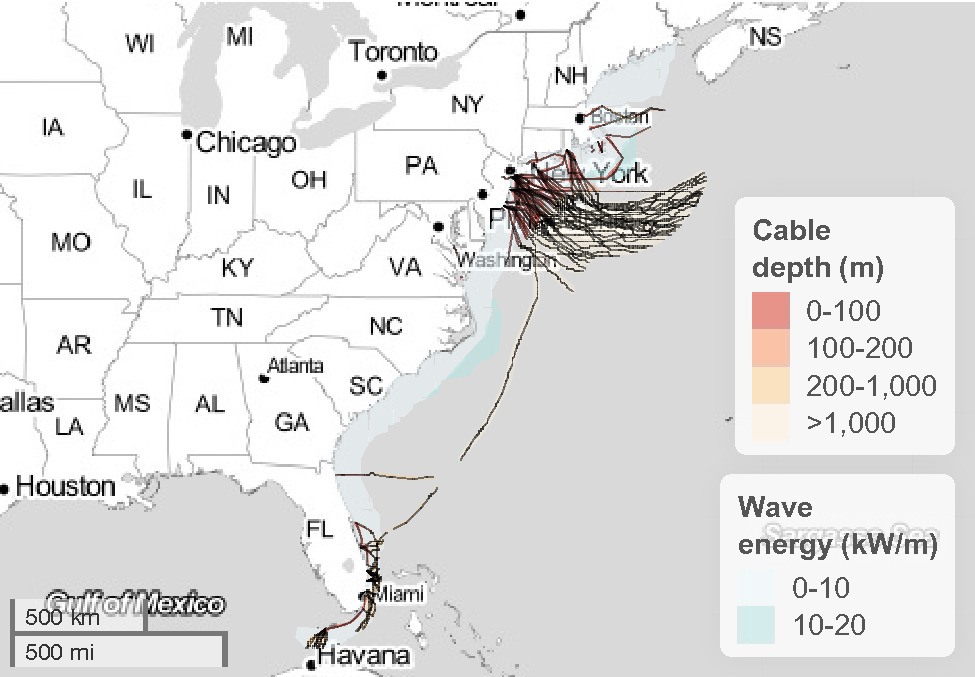
\includegraphics{report_files/figure-latex/mapWaveEast-1.pdf}
\caption{\label{fig:mapWaveEast}Map of wave energy (\(kW/m\)) in the East
with submarine cables (black lines) and advisory buffers colored by
bottom depth. The buffers are plotted with transparency so the inner
more opaque band represents the advised horizontal separation scheme for
new facilities (2 * depth) and outer less opaque band the scheme for new
cables (3 * depth). At large scales this detail is not visible.
Alternatively, you can zoom and pan interactively on these layers at
\url{http://ecoquants.github.io/nrel-cables/maps.html}.}
\end{figure}

\hypertarget{gulf-of-mexico-1}{%
\subsubsection{Gulf of Mexico}\label{gulf-of-mexico-1}}

\begin{figure}
\centering
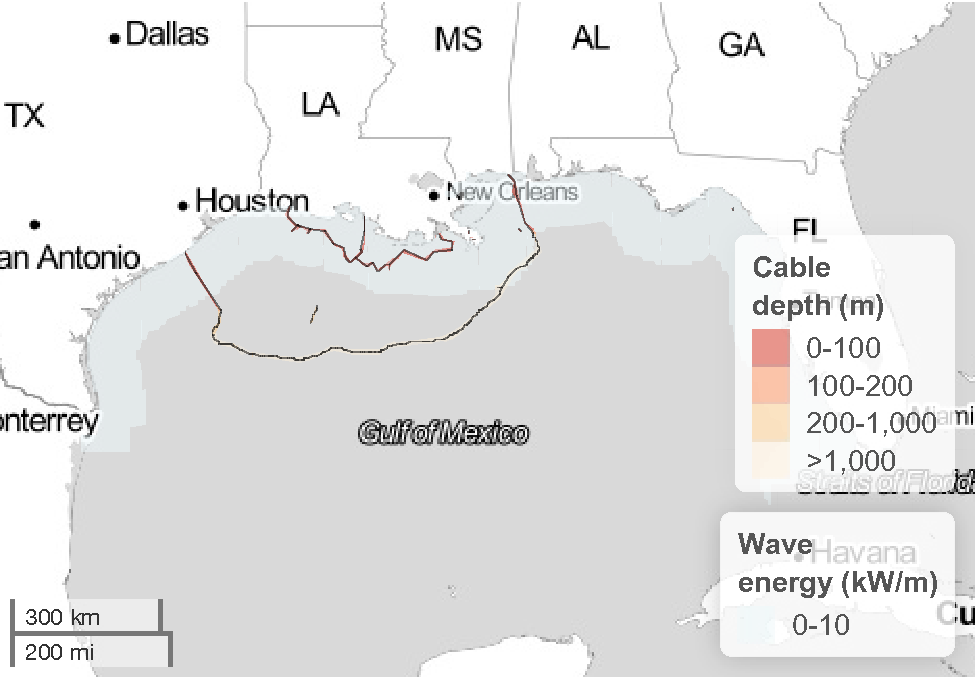
\includegraphics{report_files/figure-latex/mapWaveGulfofMexico-1.pdf}
\caption{\label{fig:mapWaveGulfofMexico}Map of wave energy (\(kW/m\)) in the
Gulf of Mexico with submarine cables (black lines) and advisory buffers
colored by bottom depth. The buffers are plotted with transparency so
the inner more opaque band represents the advised horizontal separation
scheme for new facilities (2 * depth) and outer less opaque band the
scheme for new cables (3 * depth). At large scales this detail is not
visible. Alternatively, you can zoom and pan interactively on these
layers at \url{http://ecoquants.github.io/nrel-cables/maps.html}.}
\end{figure}

\hypertarget{hawaii}{%
\subsubsection{Hawaii}\label{hawaii}}

\begin{figure}
\centering
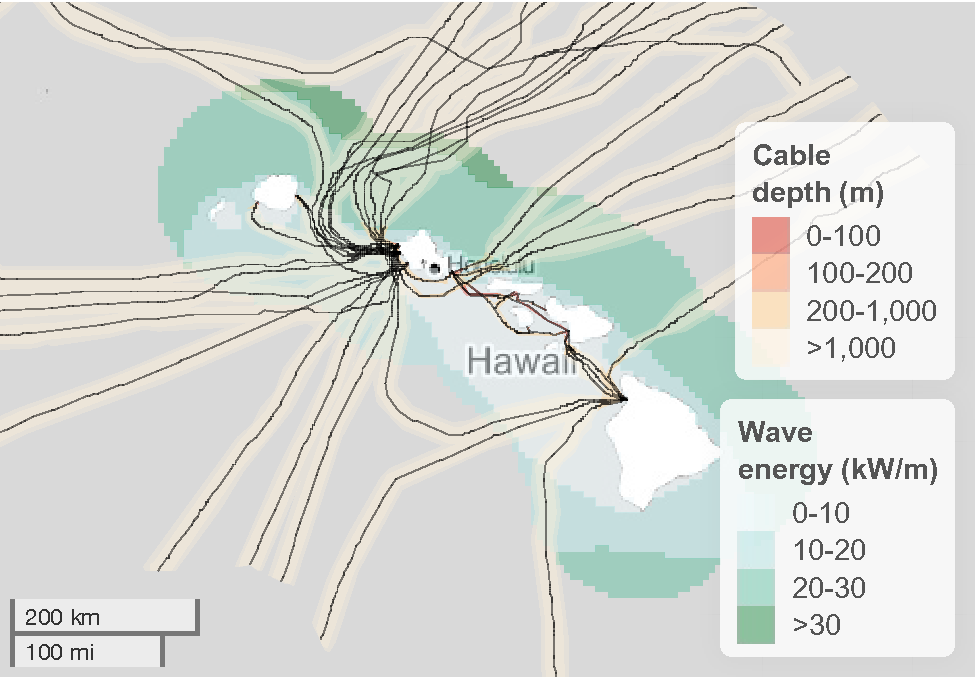
\includegraphics{report_files/figure-latex/mapWaveHawaii-1.pdf}
\caption{\label{fig:mapWaveHawaii}Map of wave energy (\(kW/m\)) in Hawaii
with submarine cables (black lines) and advisory buffers colored by
bottom depth. The buffers are plotted with transparency so the inner
more opaque band represents the advised horizontal separation scheme for
new facilities (2 * depth) and outer less opaque band the scheme for new
cables (3 * depth). At large scales this detail is not visible.
Alternatively, you can zoom and pan interactively on these layers at
\url{http://ecoquants.github.io/nrel-cables/maps.html}.}
\end{figure}

\hypertarget{puerto-rico-1}{%
\subsubsection{Puerto Rico}\label{puerto-rico-1}}

\begin{figure}
\centering
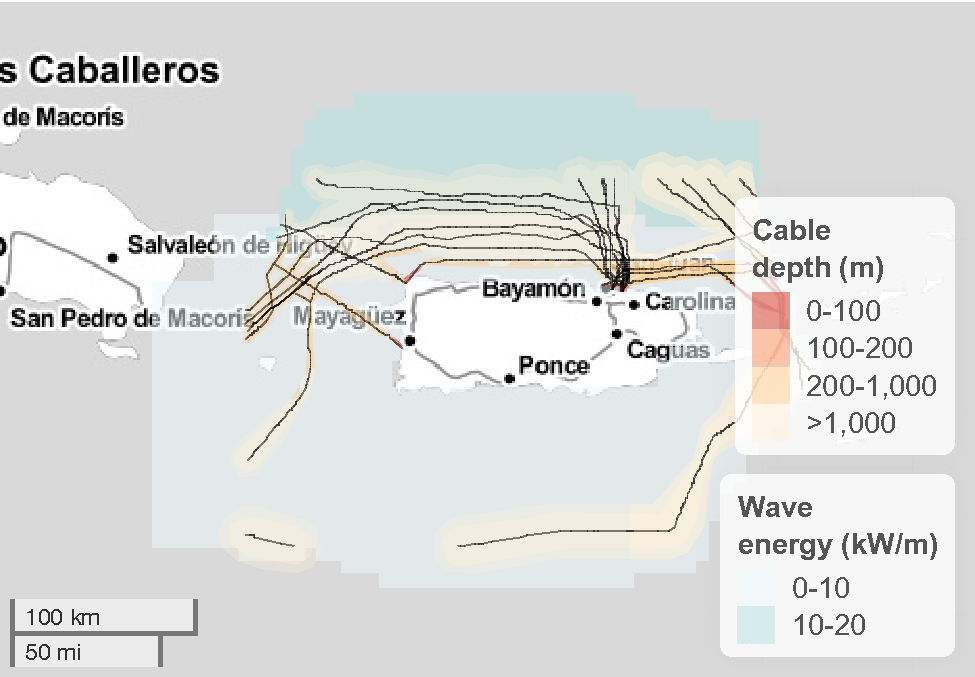
\includegraphics{report_files/figure-latex/mapWavePuertoRico-1.pdf}
\caption{\label{fig:mapWavePuertoRico}Map of wave energy (\(kW/m\)) in
Puerto Rico with submarine cables (black lines) and advisory buffers
colored by bottom depth. The buffers are plotted with transparency so
the inner more opaque band represents the advised horizontal separation
scheme for new facilities (2 * depth) and outer less opaque band the
scheme for new cables (3 * depth). At large scales this detail is not
visible. Alternatively, you can zoom and pan interactively on these
layers at \url{http://ecoquants.github.io/nrel-cables/maps.html}.}
\end{figure}

\hypertarget{us-virgin-islands-1}{%
\subsubsection{US Virgin Islands}\label{us-virgin-islands-1}}

\begin{figure}
\centering
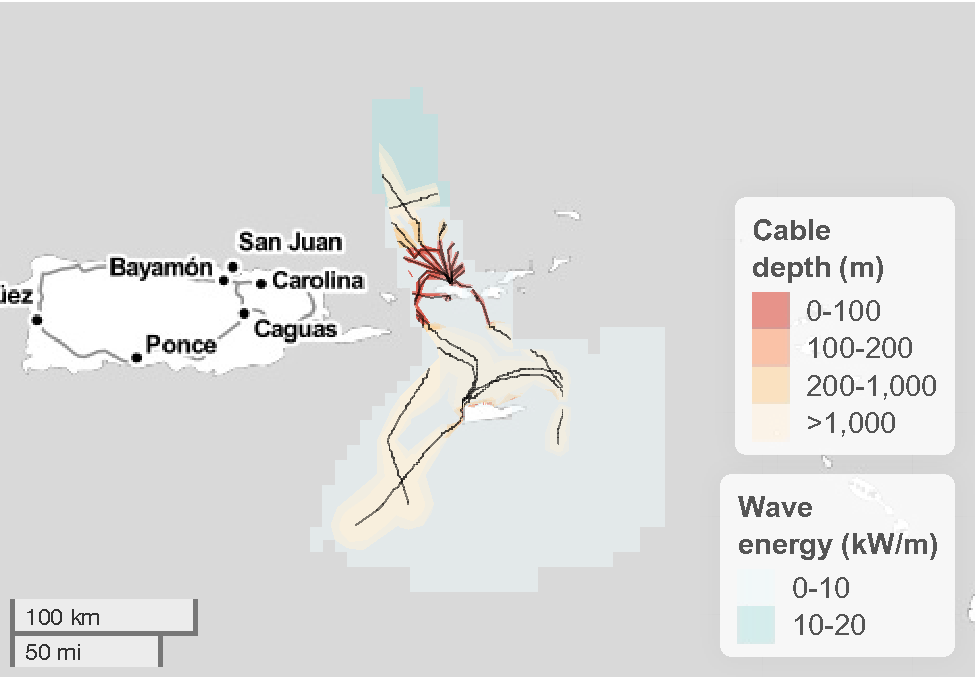
\includegraphics{report_files/figure-latex/mapWaveUSVirginIslands-1.pdf}
\caption{\label{fig:mapWaveUSVirginIslands}Map of wave energy (\(kW/m\)) in
the US Virgin Islands with submarine cables (black lines) and advisory
buffers colored by bottom depth. The buffers are plotted with
transparency so the inner more opaque band represents the advised
horizontal separation scheme for new facilities (2 * depth) and outer
less opaque band the scheme for new cables (3 * depth). At large scales
this detail is not visible. Alternatively, you can zoom and pan
interactively on these layers at
\url{http://ecoquants.github.io/nrel-cables/maps.html}.}
\end{figure}

\hypertarget{west-1}{%
\subsubsection{West}\label{west-1}}

\begin{figure}
\centering
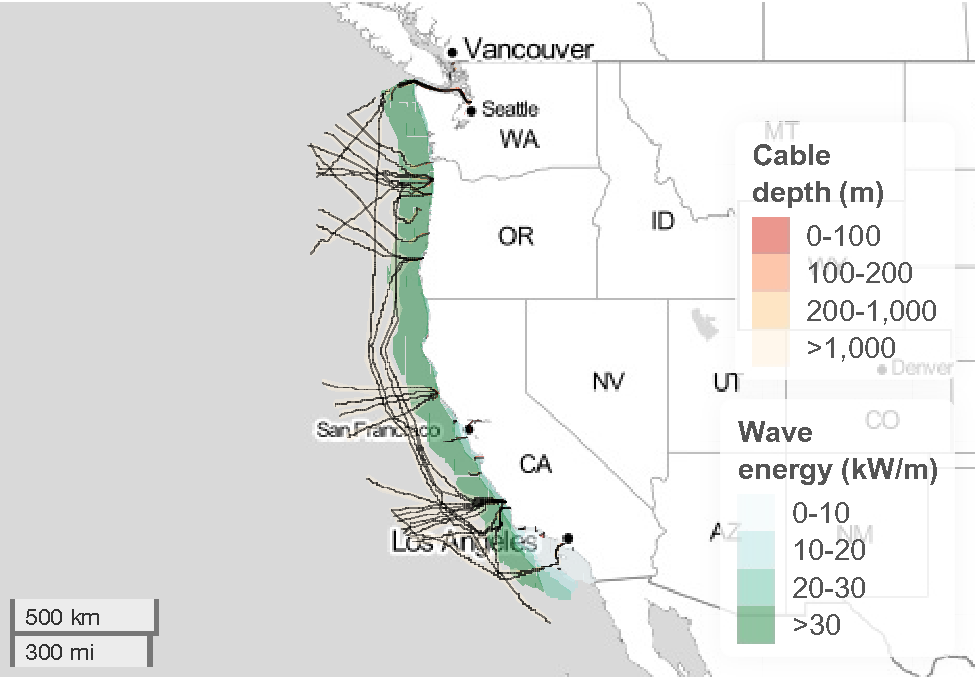
\includegraphics{report_files/figure-latex/mapWaveWest-1.pdf}
\caption{\label{fig:mapWaveWest}Map of wave energy (\(kW/m\)) in the West
with submarine cables (black lines) and advisory buffers colored by
bottom depth. The buffers are plotted with transparency so the inner
more opaque band represents the advised horizontal separation scheme for
new facilities (2 * depth) and outer less opaque band the scheme for new
cables (3 * depth). At large scales this detail is not visible.
Alternatively, you can zoom and pan interactively on these layers at
\url{http://ecoquants.github.io/nrel-cables/maps.html}.}
\end{figure}

\hypertarget{wind-1}{%
\subsection{Wind}\label{wind-1}}

\hypertarget{east-2}{%
\subsubsection{East}\label{east-2}}

\begin{figure}
\centering
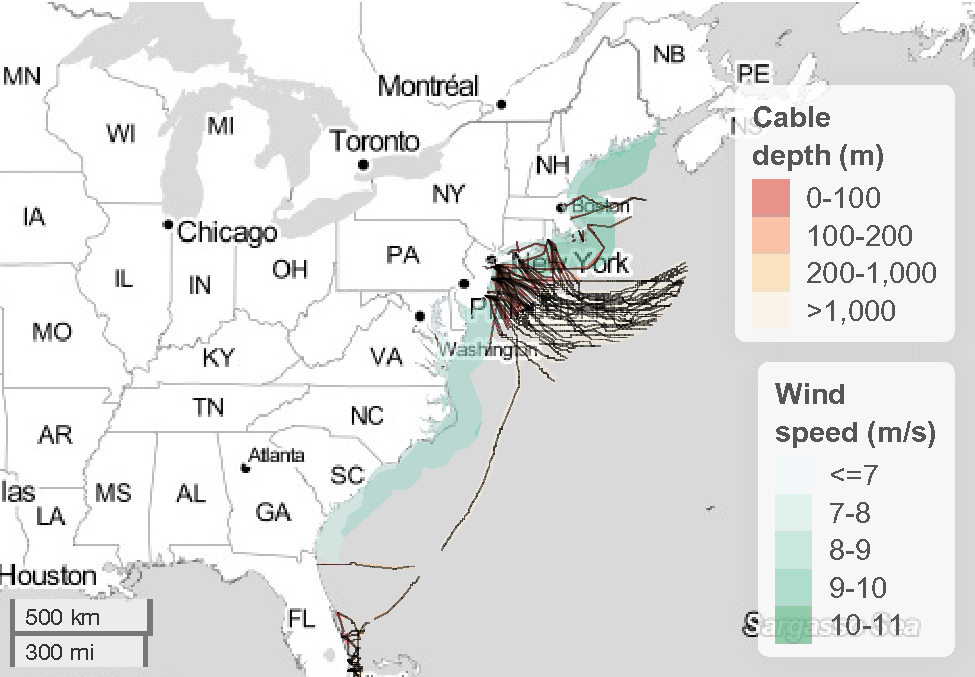
\includegraphics{report_files/figure-latex/mapWindEast-1.pdf}
\caption{\label{fig:mapWindEast}Map of wind speed (\(m/s\)) in the East with
submarine cables (black lines) and advisory buffers colored by bottom
depth. The buffers are plotted with transparency so the inner more
opaque band represents the advised horizontal separation scheme for new
facilities (2 * depth) and outer less opaque band the scheme for new
cables (3 * depth). At large scales this detail is not visible.
Alternatively, you can zoom and pan interactively on these layers at
\url{http://ecoquants.github.io/nrel-cables/maps.html}.}
\end{figure}

\hypertarget{gulf-of-mexico-2}{%
\subsubsection{Gulf of Mexico}\label{gulf-of-mexico-2}}

\begin{figure}
\centering
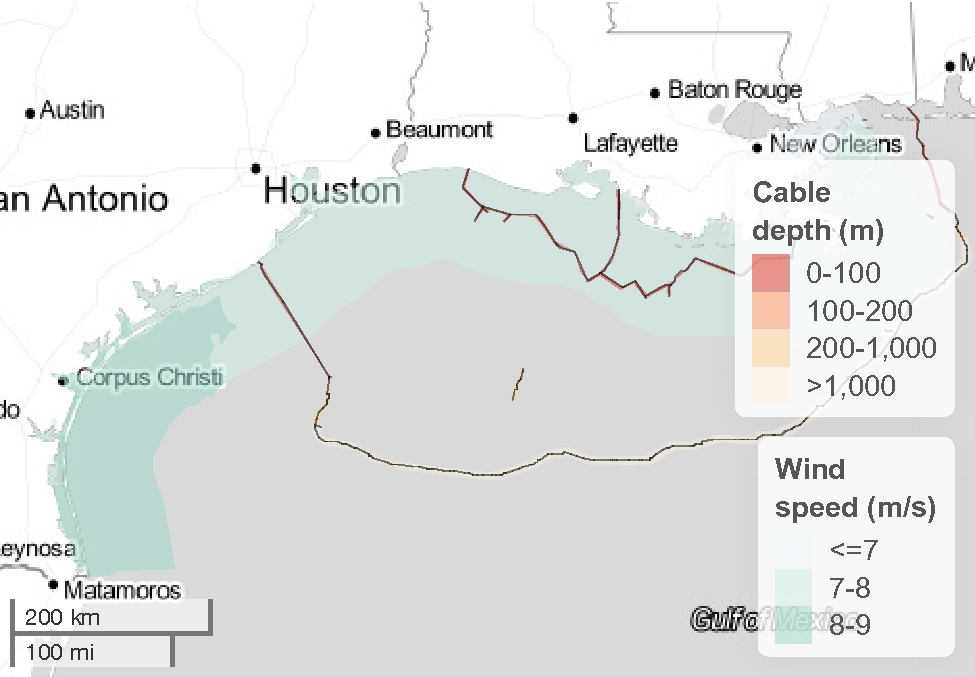
\includegraphics{report_files/figure-latex/mapWindGulfofMexico-1.pdf}
\caption{\label{fig:mapWindGulfofMexico}Map of wind speed (\(m/s\)) in the
Gulf of Mexico with submarine cables (black lines) and advisory buffers
colored by bottom depth. The buffers are plotted with transparency so
the inner more opaque band represents the advised horizontal separation
scheme for new facilities (2 * depth) and outer less opaque band the
scheme for new cables (3 * depth). At large scales this detail is not
visible. Alternatively, you can zoom and pan interactively on these
layers at \url{http://ecoquants.github.io/nrel-cables/maps.html}.}
\end{figure}

\hypertarget{hawaii-1}{%
\subsubsection{Hawaii}\label{hawaii-1}}

\begin{figure}
\centering
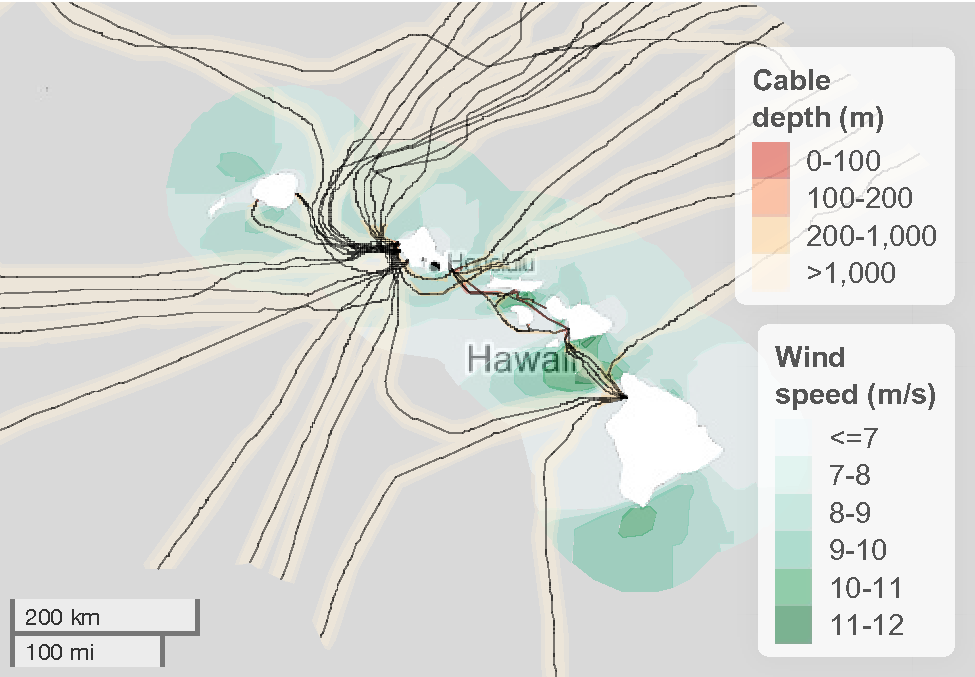
\includegraphics{report_files/figure-latex/mapWindHawaii-1.pdf}
\caption{\label{fig:mapWindHawaii}Map of wind speed (\(m/s\)) in Hawaii with
submarine cables (black lines) and advisory buffers colored by bottom
depth. The buffers are plotted with transparency so the inner more
opaque band represents the advised horizontal separation scheme for new
facilities (2 * depth) and outer less opaque band the scheme for new
cables (3 * depth). At large scales this detail is not visible.
Alternatively, you can zoom and pan interactively on these layers at
\url{http://ecoquants.github.io/nrel-cables/maps.html}.}
\end{figure}

\hypertarget{west-2}{%
\subsubsection{West}\label{west-2}}

\begin{figure}
\centering
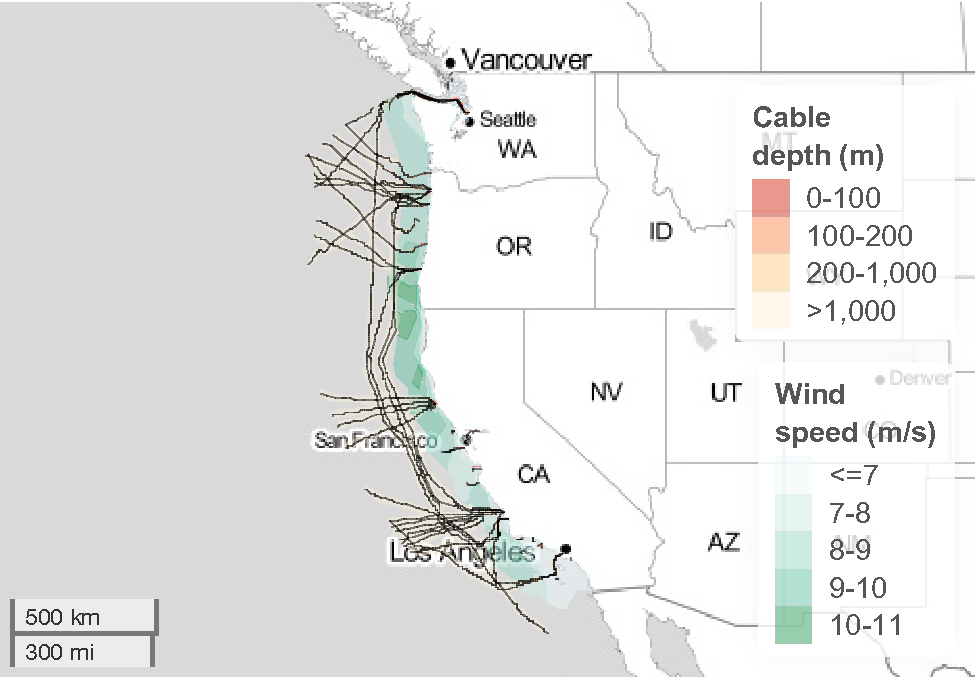
\includegraphics{report_files/figure-latex/mapWindWest-1.pdf}
\caption{\label{fig:mapWindWest}Map of wind speed (\(m/s\)) in the West with
submarine cables (black lines) and advisory buffers colored by bottom
depth. The buffers are plotted with transparency so the inner more
opaque band represents the advised horizontal separation scheme for new
facilities (2 * depth) and outer less opaque band the scheme for new
cables (3 * depth). At large scales this detail is not visible.
Alternatively, you can zoom and pan interactively on these layers at
\url{http://ecoquants.github.io/nrel-cables/maps.html}.}
\end{figure}

\newpage

\hypertarget{references}{%
\section*{References}\label{references}}
\addcontentsline{toc}{section}{References}

\hypertarget{refs}{}
\leavevmode\hypertarget{ref-beiter_assessment_2017}{}%
Beiter, P., Musial, W., Kilcher, L., Maness, M., \& Smith, A. (2017).
\emph{An Assessment of the Economic Potential of Offshore Wind in the
United States from 2015 to 2030}. NREL (National Renewable Energy
Laboratory (NREL), Golden, CO (United States)).
\url{https://tethys.pnnl.gov/sites/default/files/publications/Beiter-et-al-2017-NETL.pdf}

\leavevmode\hypertarget{ref-communicationssecurityreliabilityandinteroperabilitycounciliv_protection_2014}{}%
Communications Security, Reliability and Interoperability Council IV.
(2014). \emph{Protection of Submarine Cables Through Spatial
Separation}.
\url{http://transition.fcc.gov/pshs/advisory/csric4/CSRIC_IV_WG8_Report1_3Dec2014.pdf}

\leavevmode\hypertarget{ref-communicationssecurityreliabilityandinteroperabilitycounciliv_clustering_2016}{}%
Communications Security, Reliability and Interoperability Council IV.
(2016). \emph{Clustering of Cables and Cable Landings}.

\leavevmode\hypertarget{ref-flandersmarineinstitute_maritime_2016}{}%
Flanders Marine Institute. (2016). Maritime Boundaries Geodatabase:
Maritime Boundaries and Exclusive Economic Zones (200NM), version 9.
\url{http://www.marineregions.org/}. Accessed 25 April 2017

\leavevmode\hypertarget{ref-gilman_national_2016}{}%
Gilman, P., Maurer, B., Feinberg, L., Duerr, A., Peterson, L., Musial,
W., et al. (2016). \emph{National Offshore Wind Strategy: Facilitating
the Development of the Offshore Wind Industry in the United States.}
Office of Energy Efficiency; Renewable Energy (EERE), Washington, DC
(United States).
\url{https://www.boem.gov/National-Offshore-Wind-Strategy/}

\leavevmode\hypertarget{ref-haas_assessment_2011}{}%
Haas, K. A., Fritz, H. M., French, S. P., Smith, B. T., \& Neary, V.
(2011). \emph{Assessment of energy production potential from tidal
streams in the United States}. Georgia Tech Research Corporation,
Atlanta, GA (United States).
\url{https://www.osti.gov/scitech/servlets/purl/1219367}

\leavevmode\hypertarget{ref-Jacobson_Hagerman_Scott_2011}{}%
Jacobson, P. T., Hagerman, G., \& Scott, G. (2011). \emph{Mapping and
Assessment of the United States Ocean Wave Energy Resource}.
\url{http://www.osti.gov/scitech/servlets/purl/1060943}

\leavevmode\hypertarget{ref-lehmann_ocean_2017a}{}%
Lehmann, M., Karimpour, F., Goudey, C. A., Jacobson, P. T., \& Alam,
M.-R. (2017). Ocean wave energy in the United States: Current status and
future perspectives. \emph{Renewable and Sustainable Energy Reviews},
\emph{74}, 1300--1313.
doi:\href{https://doi.org/10.1016/j.rser.2016.11.101}{10.1016/j.rser.2016.11.101}

\leavevmode\hypertarget{ref-lowndes_our_2017}{}%
Lowndes, J. S. S., Best, B. D., Scarborough, C., Afflerbach, J. C.,
Frazier, M. R., O'Hara, C. C., et al. (2017). Our path to better science
in less time using open data science tools. \emph{Nature Ecology \&
Evolution}, \emph{1}(6), 160.
doi:\href{https://doi.org/10.1038/s41559-017-0160}{10.1038/s41559-017-0160}

\leavevmode\hypertarget{ref-madeyski_reproducible_2015}{}%
Madeyski, L., \& Kitchenham, B. (2015). Reproducible researchwhat, why
and how. \emph{Wroclaw University of Technology, PRE W}, \emph{8}.
\url{http://madeyski.e-informatyka.pl/download/MadeyskiKitchenham15.pdf}.
Accessed 3 October 2017

\leavevmode\hypertarget{ref-musial_2016_2016}{}%
Musial, W., Heimiller, D., Beiter, P., Scott, G., \& Draxl, C. (2016).
\emph{2016 Offshore Wind Energy Resource Assessment for the United
States}. NREL (National Renewable Energy Laboratory (NREL), Golden, CO
(United States)). \url{http://www.nrel.gov/docs/fy16osti/66599.pdf}

\leavevmode\hypertarget{ref-pachauri_climate_2015}{}%
Pachauri, R. K., Mayer, L., \& Intergovernmental Panel on Climate Change
(Eds.). (2015). \emph{Climate change 2014: Synthesis report}. Geneva,
Switzerland: Intergovernmental Panel on Climate Change.

\leavevmode\hypertarget{ref-schwartz_assessment_2010a}{}%
Schwartz, M., Heimiller, D., Haymes, S., \& Musial, W. (2010).
\emph{Assessment of offshore wind energy resources for the United
States}. National Renewable Energy Laboratory (NREL), Golden, CO.
\url{https://pdfs.semanticscholar.org/ee6a/c56b0ff8a7c56c575cf774001a9f27490907.pdf}

\leavevmode\hypertarget{ref-uihlein_wave_2016}{}%
Uihlein, A., \& Magagna, D. (2016). Wave and tidal current energy review
of the current state of research beyond technology. \emph{Renewable and
Sustainable Energy Reviews}, \emph{58}, 1070--1081.
\url{http://www.sciencedirect.com/science/article/pii/S1364032115016676}

\leavevmode\hypertarget{ref-vliz_iho_2017}{}%
VLIZ. (2017). IHO Sea Areas, version 2. VLIZ.
\url{http://www.marineregions.org/}. Accessed 2 July 2017

\leavevmode\hypertarget{ref-weatherall_new_2015}{}%
Weatherall, P., Marks, K. M., Jakobsson, M., Schmitt, T., Tani, S.,
Arndt, J. E., et al. (2015). A new digital bathymetric model of the
world's oceans. \emph{Earth and Space Science}, \emph{2}(8),
2015EA000107.
doi:\href{https://doi.org/10.1002/2015EA000107}{10.1002/2015EA000107}


\end{document}
